\chapter{\nmu Modélisation long terme de signaux sonores} \label{chap:modeles}

La plupart des modèles de sons utilisés dans la littérature sont des modèles à court terme, c'est-à-dire qu'ils modélisent le signal sur une courte période de temps. Les raisons de ce choix de conception sont nombreuses et seront détaillées ci-après. Une originalité de mon travail de recherche a été d'étudier les limitations de ce type d'approche et de contribuer à des alternatives qui, sans être totalement satisfaisantes à ce jour, nous permettent de mieux comprendre les défis scientifiques et techniques pour parvenir à une modélisation des signaux sonores qui soit à la fois fidèle, versatile, et expressive.

\section{ \nmu Préambule}

On considérera ici qu'un signal sonore est un signal à valeurs réelles, échantillonné à une fréquence de 40 kHz environ. \`A titre d'exemple, la Figure \ref{fig:onde} montre la forme d'onde d'une note de piano. Ce signal peut provenir d'une version quantifiée, mais on supposera que le pas de quantification est suffisamment réduit pour n'introduire qu'une dégradation perceptivement négligeable. On notera ce signal $x[n]$. Il peut être observé sur un intervalle de temps donné, correspondant à un certain nombre d'échantillons temporels $x[n], n \in [1, ..., N]$ souvent appelé intervalle d'observation, trame, support ou encore champ réceptif. Je n'utiliserai pas dans ce document la version continue du signal, l'expression $f(x)$ devant se comprendre comme l'application d'une fonction $f$ à un signal $x$.

\begin{marginfigure}
  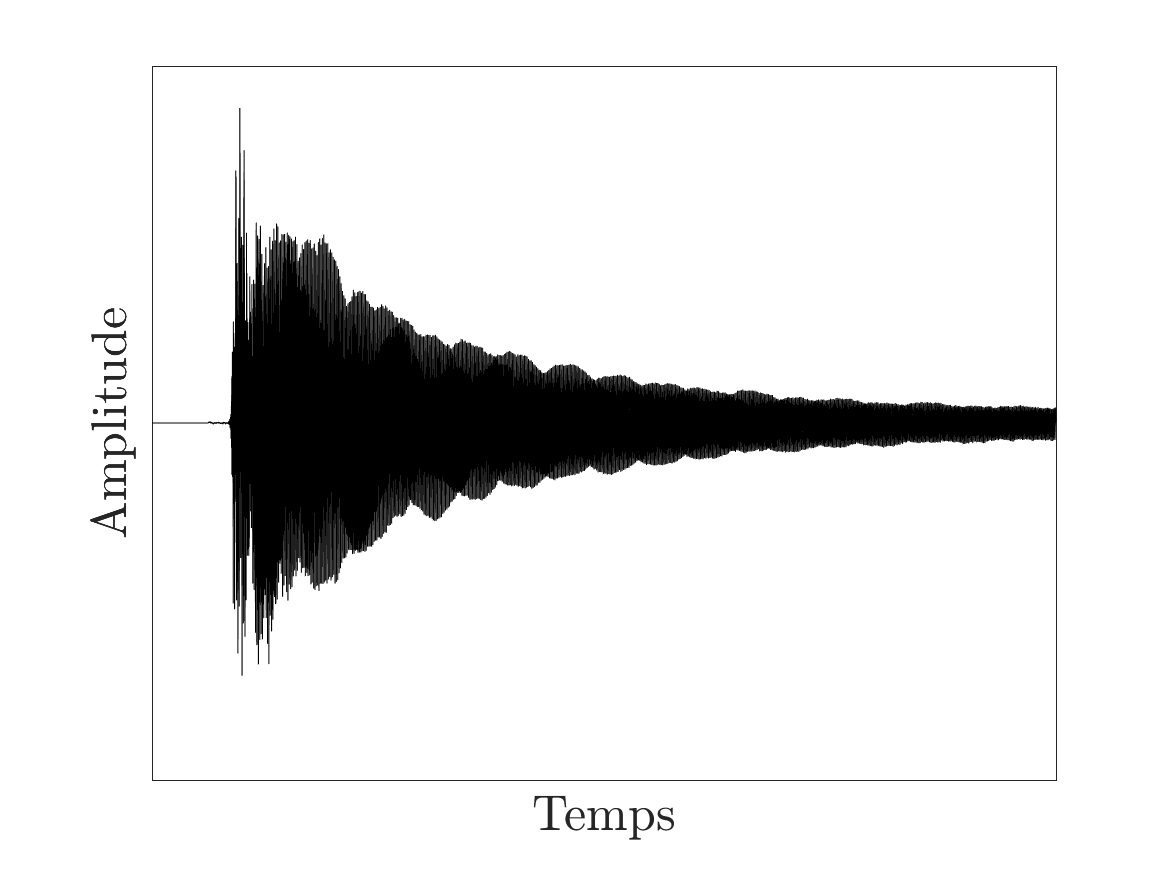
\includegraphics[width=\textwidth]{pianoGray}
  \caption{Signal temporel ou forme d'onde d'une note de piano.}
  \label{fig:onde}
\end{marginfigure}

Le terme modélisation étant fortement polysémique, précisons l'usage qui sera fait du terme \og modèle de son \fg. Un modèle de son est une représentation du signal sonore qui permet de modifier ce signal d'une manière qui soit d'intérêt pour une tâche donnée et ce de manière cohérente avec certaines contraintes motivées par 1) des considérations physiques ou 2) la perception qu'en aurait un être humain. On notera $\mathrm{Pe}(x)$, l'opérateur de perception humaine du signal $x$.  Le modèle est utilisé en considérant deux étapes de transformation, respectivement appelées \og analyse \fg et \og synthèse \fg. La phase d'analyse $\mathrm{An}$, à partir d'un signal $x$, produit un modèle $X$ et la phase de synthèse $\mathrm{Sy}$ permet, à partir de ce modèle $X$, de produire un signal $\tilde{x}=\mathrm{Sy}(\mathrm{An}(x))$.

Trois critères d'évaluation sont d'importance pour qualifier ce modèle pour des activités de conception, création et manipulation :
\begin{enumerate}
  \item\textbf{fidélité} : un modèle fidèle est capable de ne pas produire d'artefacts. Ce critère peut s'exprimer formellement de la manière suivante : $\mathrm{Pe}(x) \sim \mathrm{Pe}(\tilde{x})$.
  \item\textbf{expressivité} : un modèle expressif est capable de mettre à disposition des mécanismes de manipulation tels que la modification du modèle produise une modification cohérente de la perception du signal résultant. Ce critère peut s'exprimer formellement de la manière suivante : $\mathrm{Pe}(\mathrm{Sy}(X')) \sim \mathrm{Pe}(x')$, où $X'$ désigne une version du modèle $X$ modifié avec des opérateurs simples, et $x'$ désigne une version modifiée du signal $x$ à partir d'opérateurs complexes: étirement, transposition, etc.
  \item\textbf{versatilité} : un modèle versatile s'applique à tout type de signal sonore d'intérêt, \textit{i.e.} les conditions de fidélité et d'expressivité sont remplies pour tout signal $x$ d'intérêt pour une tâche donnée.
\end{enumerate}
Je ne considère pas ici la notion d'efficacité, \textit{i.e.} la capacité à modéliser des signaux avec peu de paramètres. Cette notion sera un élément prépondérant d'évaluation par exemple pour un algorithme de compression. De par mon expérience, les notions d'expressivité et d'efficacité sont subtilement liées. Il est néanmoins important de noter qu'un modèle efficace n'est pas forcément expressif, et qu'un modèle expressif n'est pas forcément efficace.

L'expressivité sera évaluée ici au regard des modifications canoniques du signal sonore, à savoir:
\begin{itemize}
  \item la modification du volume;
  \item la modification de la durée;
  \item la modification de la hauteur;
  \item la modification du timbre.
\end{itemize}
Bien d'autres peuvent être imaginées ou désirées, en fonction de projets de création spécifiques.

\marginnote{
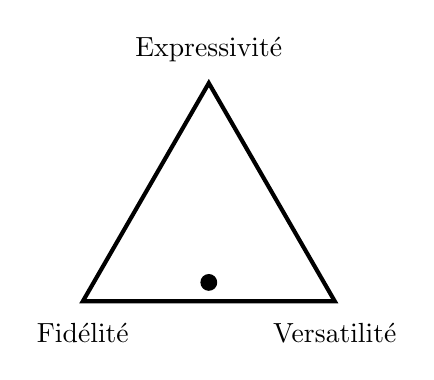
\begin{tikzpicture}[scale=0.8, label distance=1.5mm]
    \coordinate[label=below:Fidélité]  (A) at (0,0);
    \coordinate[label=below:Versatilité] (B) at (4,0);
    \coordinate[label=above:Expressivité] (C) at (2,3.464);
    \draw [line width=1.5pt] (A) -- (B) -- (C) -- cycle;
    \draw [black, fill=black, line width=1.5pt] (2,.3) circle [radius=.1 cm]; % raw
  \end{tikzpicture}
  La forme d'onde est modèle de son versatile et fidèle mais d'une expressivité limitée.
}
Avec ces trois critères d'évaluation, se dessine ici un triangle de contraintes qui nous permettra d'apprécier le compromis inhérent au choix de conception de chacun des modèles que nous discuterons. Par exemple, la forme d'onde est un modèle versatile et fidèle mais d'une expressivité limitée, car il n'y a guère que le volume que l'on puisse manipuler aisément.

L'intuition ici, largement suivie dans la communauté des sciences des données est que, pour tout processus observable, il existe un modèle de ce processus pour lequel des manipulations basées sur des opérateurs mathématiques simples dans le domaine transformé \og font sens \fg dans le domaine signal. On jugera alors la qualité du modèle par sa capacité à proposer de nouvelles réalisations du processus modélisé qui soient plausibles, dans notre cas perceptivement valides. Par exemple, en considérant le signal temporel, on peut aisément manipuler l'intensité perçue en multipliant tous les échantillons par une constante. Ce modèle ne permet par contre pas dans le cas général de manipuler aisément la hauteur perçue.

Cette approche se distingue clairement des approches par \og modèle physique \fg qui modélisent explicitement le processus mécanique, la qualité du son étant alors censée être la résultante d'une bonne modélisation du système physique dont la mise en vibration est à l'origine du signal sonore d'intérêt. Le distinguo est ici fait sur l'objet d'intérêt, à savoir que l'on s'intéresse aux propriétés du signal et non à celles de la source. Ceci ne veut pas dire que l'on ne puisse pas, avec une approche sciences des données, se focaliser sur le signal d'un type de source sonore en particulier. Mais, dans ce cas, on s'attachera à exploiter les régularités du signal pour motiver notre modèle.

Dans la communauté traitement du signal, on parle souvent de modèle paramétrique, dans le sens où le modèle dispose d'un ensemble réduit de paramètres qui peuvent être explicitement manipulés pour influer sur le son modélisé. L'usage du terme \og paramétrique \fg est malheureusement utilisé avec peu de cohérence dans la littérature. Je préférerai donc à ce terme le distinguo entre \og modèle \fg et \og transformée \fg. Un modèle expose donc pour moi un ensemble de paramètres manipulables, une transformée étant plutôt un outil de description. Ceci n'empêche pas qu'une transformée puisse avoir un modèle sous-jacent, ni que les étapes d'analyse et / ou de synthèse d'un modèle ne se basent sur une ou plusieurs transformées.

Précisons maintenant l'intervalle temporel dénommé par \og long terme \fg. Cela désignera ici une durée à partir de laquelle le signal sonore ne peut plus raisonnablement être considérée comme stationnaire. De par nos connaissances sur les propriétés physiques de l'organe phonatoire, il est par exemple commun de considérer que le signal de parole est localement stationnaire sur un intervalle de 25 ms. Comme on peut le voir en observant des spectrogrammes de vocalisations humaines,~\cite{ladefoged2014course} dès que l'on considère des consonnes, ou lorsque la prosodie évolue de manière conséquente, le signal sonore produit par l'organe vocal n'est plus stationnaire. Il me paraît donc plus juste de motiver ce choix par l'assertion suivante : \og il est raisonnable de modéliser le signal de parole avec un modèle stationnaire par morceaux à partir du moment où ces morceaux sont d'une durée inférieure à 25 ms \fg.

\marginnote[-1cm]{
  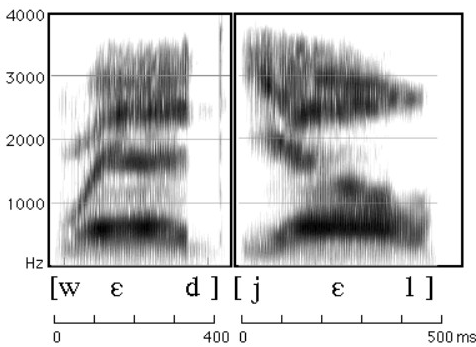
\includegraphics[width=.5\textwidth]{phonemesCrop}

Spectrogrammes de séries de phonèmes (figure issue de la référence \no 34).
 % Issue de l'ouvrage "A Course In Phonetics" de Ladefoged publié en 2006,  http://www.cog.jhu.edu/courses/325-f2004/ladefoged/course/chapter8/figure8.html
 }

La dénomination \og long terme \fg  étant dépendante du degré de stationnarité du signal étudié, il n'est donc pas possible de fixer une durée pour tout type de signaux sonores à partir de laquelle la dénomination \og long terme \fg est appropriée. On considérera néanmoins dans les études discutées dans ce document qu'un intervalle de temps  \og long terme \fg désigne un intervalle de temps supérieur ou égal à la seconde.

\section{ \nmu Typologie sonore} \label{sec:typologie}

Il est bien entendu que même si l'on souhaite que notre modèle soit versatile, on ne souhaite pas être capable de modéliser tous les signaux possibles. On supposera donc que certaines propriétés d'invariance existent, c'est-à-dire que même si une seconde de son échantillonné à 44 kHz est représentée dans $R^{44000}$, les paramètres du modèle évoluent dans un espace de dimension beaucoup plus réduit. Je considère ce postulat raisonnable essentiellement pour des raisons d'observations physiques. En prenant l'exemple du signal de parole, il est bien entendu que le son produit est le résultat d'une interaction complexe entre un ensemble d'éléments qui ont une certaine plasticité. Il reste néanmoins évident que les déformations possibles de l'ensemble de ces éléments sont bornées.

Dans le but de préciser le domaine d'investigation, je présente ici cinq grandes familles de signaux sonores :
\begin{itemize}
  \item \textbf{parole} : sons voisés <a>, <o> / sons plosifs <pe>, <qe>;
  \item \textbf{communication animale} : hululement de chouettes / clics de localisation de chauve souris;
  \item \textbf{musique} : chant lyrique / percussions;
  \item \textbf{mécanique} : ventilation / marteau piqueur;
  \item \textbf{environnementaux} : vent faisant siffler des câbles / gouttes de pluie tombant sporadiquement.
\end{itemize}\marginnote[-2cm]{Cette typologie est ordonnée par période approximative d'intérêt de la communauté de traitement du signal. Le traitement de la parole a connu un essor dans les années 1970, la bio acoustique un peu plus tard, la musique dans les années 2000 et les signaux environnementaux dans les années 2010.}

Les exemples donnés pour chaque classe sont choisis à dessein pour illustrer une dichotomie présente dans toutes ces classes. Elle nous servira de base pour notre critique des outils de modélisation à notre disposition et pour identifier les défis majeurs à relever.

Suivant cette dichotomie, certains sons portent une structuration fréquentielle forte et d'autres une structuration temporelle forte. La Figure \ref{fig:ibm} montre deux exemples dans le domaine instrumental. Ces exemples sont volontairement typés pour expliciter le propos, mais la plupart des sons naturels sont une composition de ces deux types de structures. Il est donc nécessaire pour atteindre nos objectifs de disposer d'outils performants pour modéliser conjointement ces deux types de structure, temporelle et fréquentielle.

\section{ \nmu Temps / fréquence} \label{sec:tf}

Lorsque l'on cherche à décrire un son, deux dimensions émergent : l'intensité et la hauteur. Ces deux dimensions étant respectivement intimement liés à l'amplitude et à la fréquence, il est normal de constater que la plupart des modèles de son permettent de manipuler ces deux dernières quantités de manière dynamique, \textit{i.e.} au cours du temps.



En supposant le signal sonore stationnaire sur l'intervalle d'observation, l'outil privilégié pour ce faire est la transformée de Fourier discrète (tfd). Cette transformée projette le signal sur une base d'exponentielles complexes:
\begin{eqnarray}
  X[m] &=& \sum_{n=0}^{N-1} x[n] \cdot \mathrm{e}^{\frac{-2 \mathrm{j} \pi nm}{N}} \\
  x[n] &=& \frac{1}{N} \sum_{m=0}^{N-1} X[m] \cdot \mathrm{e}^{\frac{ 2 \mathrm{j} \pi m n }{N}}.
\end{eqnarray}
Cette transformée est donc inversible, mais n'est pas à échantillonnage critique,~\footnote{Une transformée est dite à échantillonnage critique quand un signal nécessite le même nombre de bits pour être représenté dans le domaine transformé que dans celui d'origine.} car $x\in \mathbb{R}$  et $X \in \mathbb{C}$.

\begin{marginfigure}
  \begin{center}
  \footnotesize
  (a) \\
  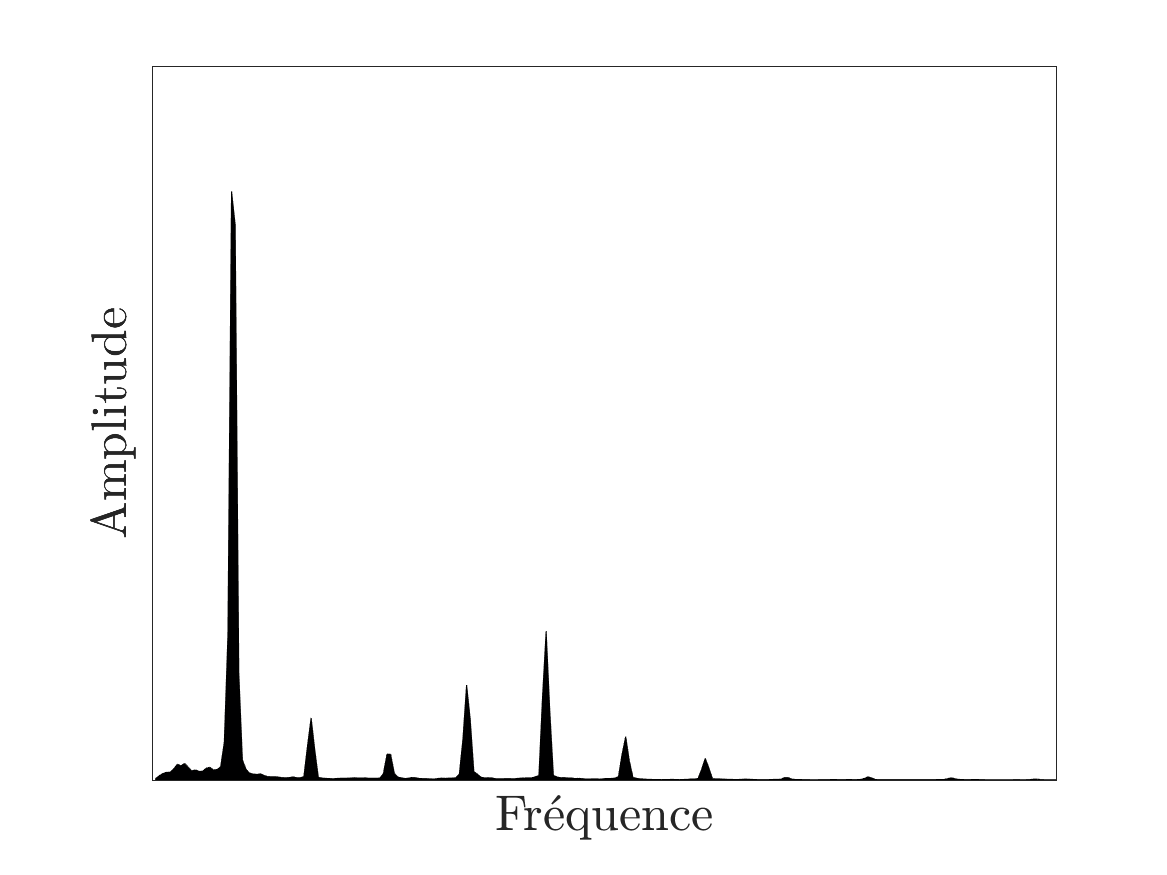
\includegraphics[width=1\textwidth]{pianoSp} \\
  (b) \\
  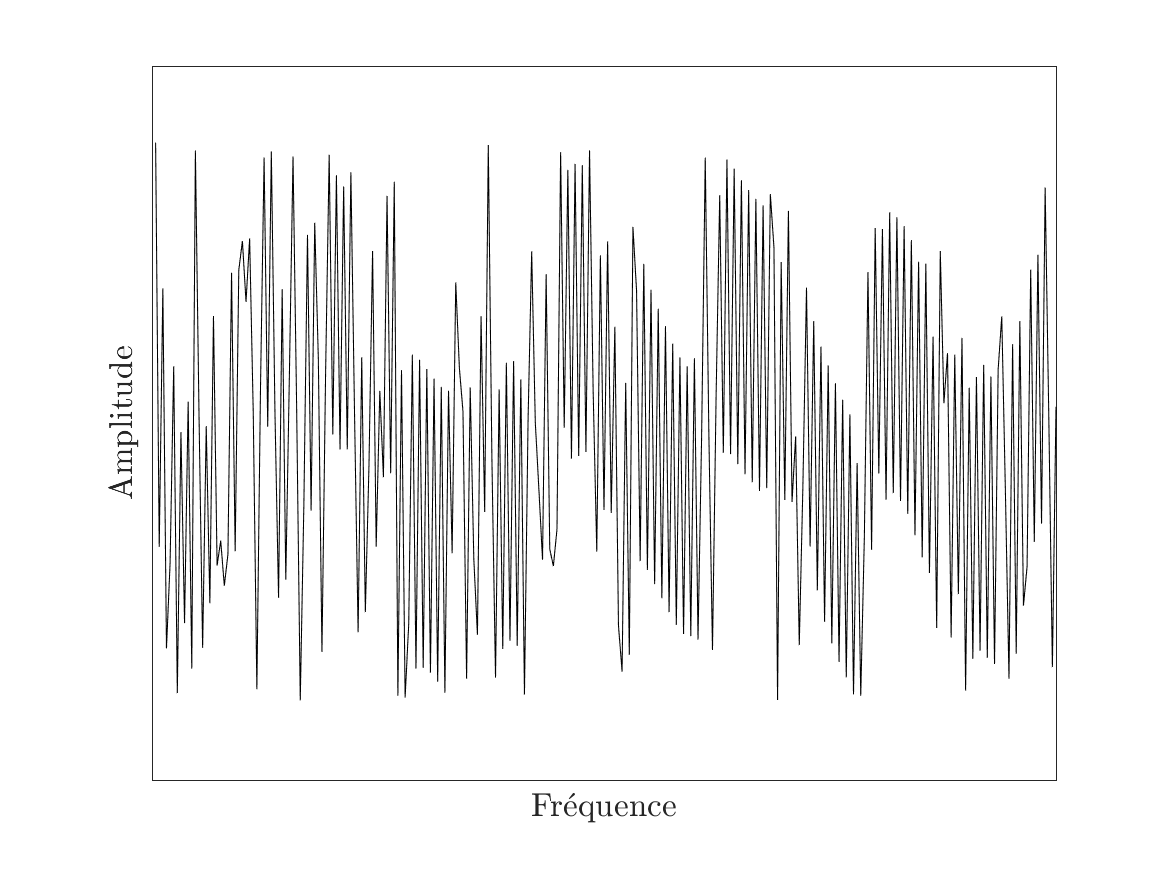
\includegraphics[width=1\textwidth]{pianoPh}
\end{center}
  \caption{Spectre d'amplitude (a) et de phase (b) d'une note de piano.}
  \label{fig:spec}
\end{marginfigure}

On calcule la transformée de Fourier de manière efficace grâce à des algorithmes de transformée de Fourier rapides qui exploitent, pour le plus connu d'entre eux, des longueurs de supports en puissance de deux.~\cite{cooley1965algorithm}



Comme on peut le voir sur la Figure \ref{fig:spec}, en considérant le module de cette transformée, on manipule directement l'intensité du son à une fréquence donnée. Le spectre de phase est lui souvent négligé dans les modèles, car il est beaucoup plus difficile à interpréter. Ceci constitue un handicap majeur pour tous les modèles de sons basés sur la transformée de Fourier car cela pose bien souvent une limite sur la propriété de fidélité, le module et l'exposant étant mathématiquement liés.


En considérant qu'une partie des sons que l'on cherche à modéliser possèdent une structure temporelle forte comme une note de piano ou un sifflement d'oiseau, on s'intéresse à l'estimation des paramètres de composantes périodiques simples, les sinusoïdes. Considérons pour cela un premier signal \og éprouvette \fg constitué d'une sinusoïde de fréquence et d'amplitude constante:
\begin{equation}
  x_s[n] = a_s \mathrm{sin}(2\pi f_s n /f_e + \phi_s)
  \label{eq:sin_toy}
\end{equation}
Les paramètres d'amplitude et de fréquence de cette composante s'estiment aisément grâce au spectre de Fourier de ce signal :
\begin{eqnarray}
  \hat{f}_s &=&  \frac{M}{N} . f_e\\
  \hat{a}_s &=& X_s[M]
    \label{eq:sin_toy_est}
\end{eqnarray}
avec
\begin{equation}
  M = \argmax_m | X_s[m] |.
  \label{eq:sin_toy_select}
\end{equation}

\marginnote[0cm]{
\footnotesize
   \begin{center}
   (a) \\
   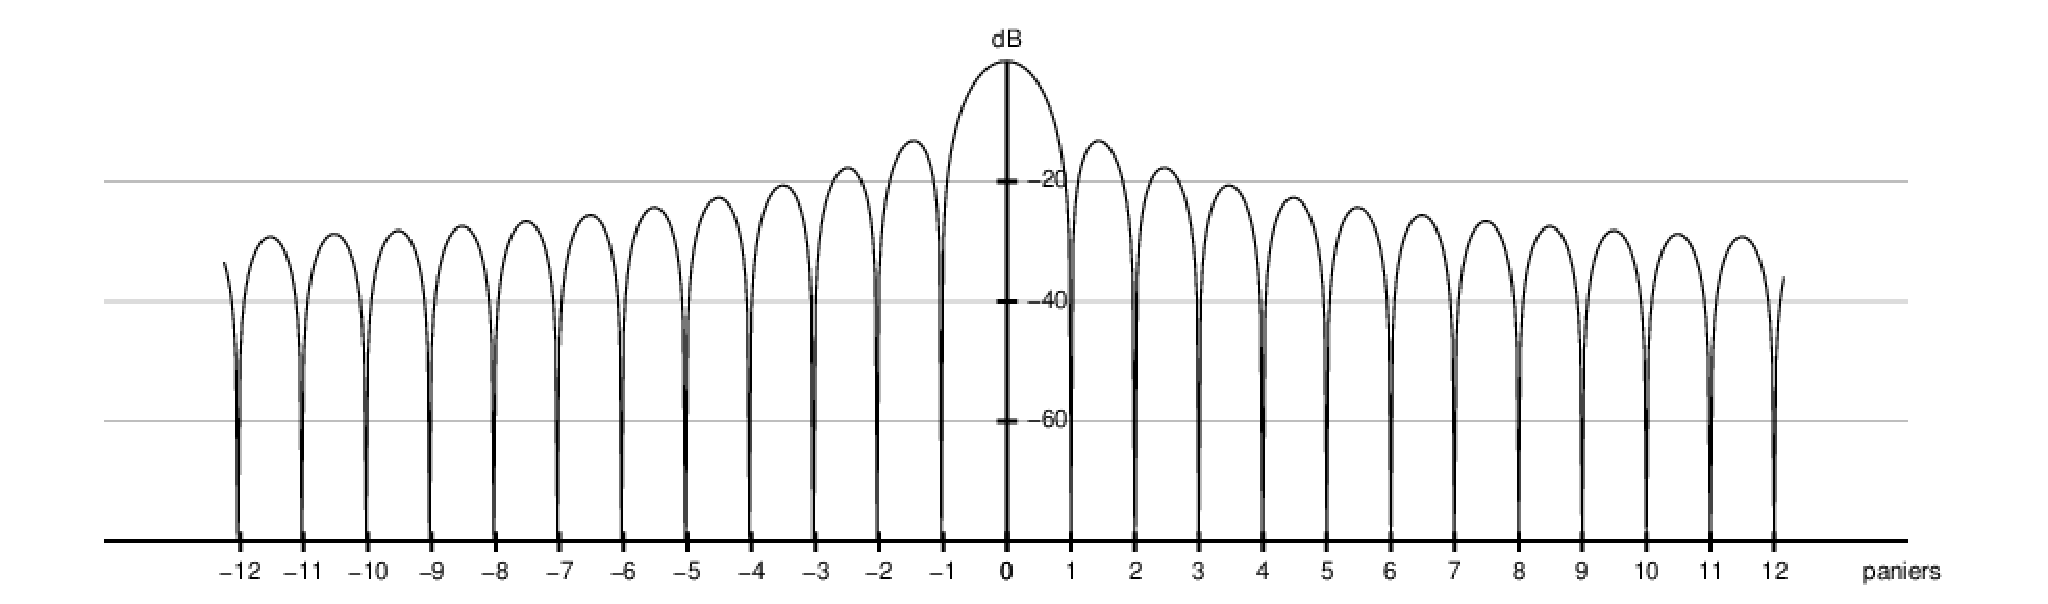
\includegraphics[width=.5\textwidth]{s-rectangularFr} \\
   (b) \\
  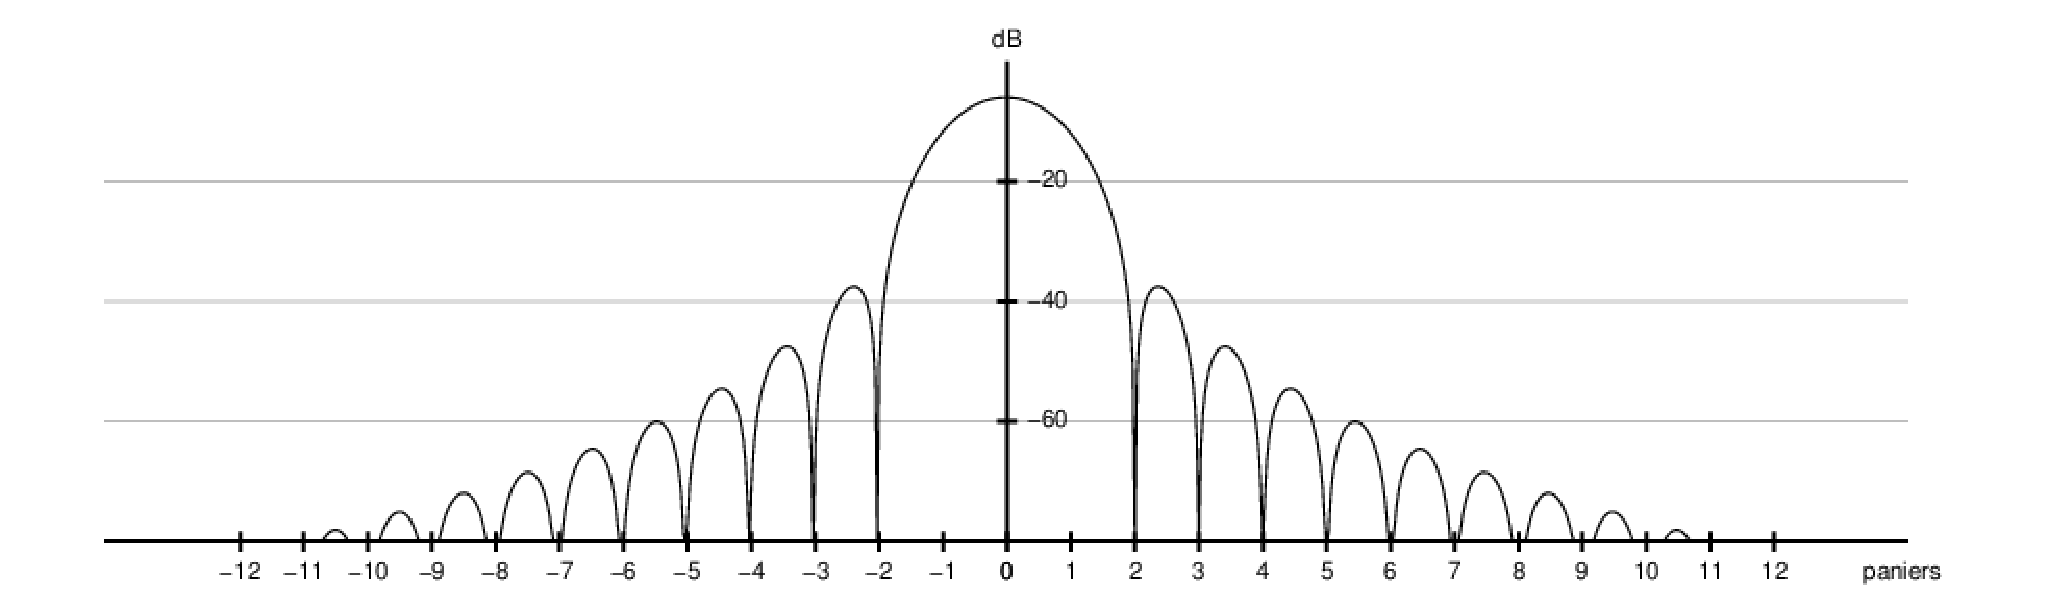
\includegraphics[width=.5\textwidth]{s-hannFr}
 \end{center}
Spectre d'amplitude de la fenêtre rectangulaire (a), et de la fenêtre de Hann (b).
}

Dans le cas de plusieurs sinusoïdes, on remplacera l'équation \ref{eq:sin_toy_select} par une sélection de maxima locaux dans le spectre de puissance et on considèrera l'usage d'une fenêtre de type co-sinusoïdale (hamming, hann, ...) pour améliorer la localité fréquentielle de la transformée.~\cite{harris1978use} En effet, considérer le signal sur un intervalle de temps fixé par la largeur de la trame revient implicitement à fenêtrer le signal par une fenêtre rectangulaire qui a des propriétés spectrales non désirables dans le cas multi composantes. Avec des fenêtres co-sinusoïdales, le lobe principal s'élargit, d'où une perte locale de résolution, mais permet de réduire considérablement l'importance des lobes secondaires, ce qui s'avère indispensable dans un contexte multi composantes.


On peut améliorer la précision de ces estimations en réduisant le pas de quantification de l'axe fréquentiel. On utilise pour cela la technique du "zero padding", qui consiste à concaténer une série de valeurs nulles au signal observé avant d'opérer la transformation. La transformée s'opérant alors sur plus de points, son pas de discrétisation fréquentielle s'en trouve augmenté. Par conséquent, la précision des estimateurs de l'équation \ref{eq:sin_toy_est} en est augmentée.

Un large échantillon de méthodes sont disponibles pour améliorer la précision de ces estimations par d'autres moyens moins directs, mais souvent plus efficaces. Celles basées sur le réassignement~\cite{auger1995improving} étudient les relations entre le spectre du signal fenêtré et le spectre du signal fenêtré par la dérivée de la fenêtre. Les méthodes basées sur la phase étudient elles les relations entre le spectre du signal et celui de sa dérivée. Ces deux méthodes, conceptuellement proches, sont en fait équivalentes théoriquement et numériquement.~\cite{lagrangeJaes07}

Il est important de bien garder en mémoire que seule la précision des estimateurs est augmentée, la résolution de la transformée restant dépendante de la largeur du support temporel.  Augmenter l'intervalle d'observation va donc non seulement influer sur la précision, mais également sur la résolution de la transformée. Ainsi, deux sinusoïdes de fréquences proches ne pourront être \og résolues \fg, c'est-à-dire que leurs paramètres ne pourront être estimés en observant directement le spectre d'amplitude que par l'extension suffisante du support temporel de la transformée. Comme nous allons le voir dans l'exemple suivant, cette extension a un coût.


\begin{marginfigure}
  \footnotesize
  \begin{center}
  (a) \\
  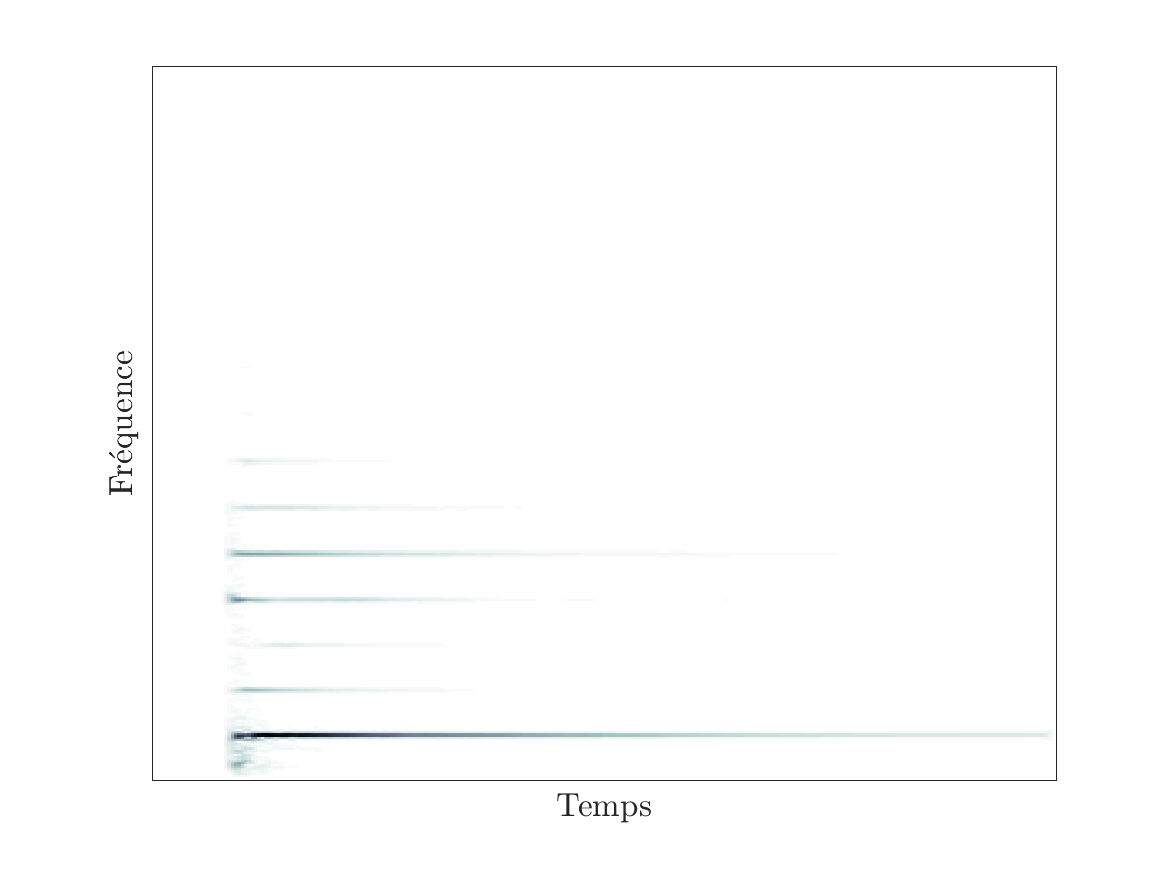
\includegraphics[width=1\textwidth]{pianoSpec} \\
  (b) \\
  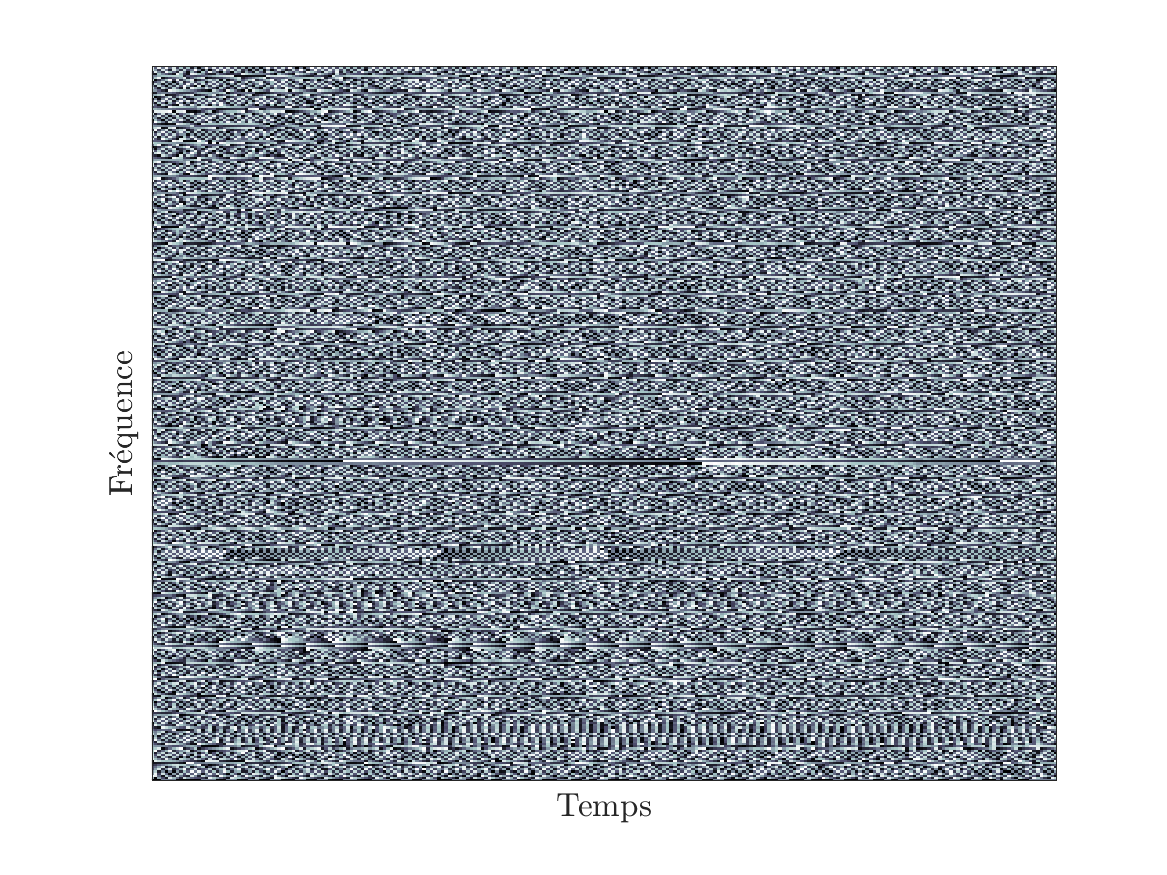
\includegraphics[width=1\textwidth]{pianoPhase} \\
\end{center}
  \caption{Spectrogramme d'amplitude (a) et de phase (b) d'une note de piano où la teinte représente la phase. TODO HSV}
  \label{fig:phase}
\end{marginfigure}

Considérons un autre signal \og éprouvette \fg constitué cette fois ci d'une impulsion de Dirac :
\begin{equation}
  s_d[n] = \begin{cases}
    a_d \text{ si } n=n_d \\
    0 \text{ sinon}
\end{cases}
\end{equation}
L'estimation du paramètre d'amplitude $a_d$ et de sa position temporelle $n_d$ est triviale dans le domaine temporel :
\begin{eqnarray}
  \hat{n_d} &=&  \argmax_n | s_d[n] | \\
  \hat{a_s} &=&  s_d[\hat{n_d}].
\end{eqnarray}

Cette dernière est par contre beaucoup plus difficile à estimer dans le domaine spectral, du fait du caractère non stationnaire du signal analysé.


Pour pallier au caractère non stationnaire à long terme de la plupart des signaux naturels, il est courant d'utiliser la transformée de Fourier à court terme (tfct). Son principe est d'effectuer une série de transformée de Fourier, chacune sur des fenêtres espacées dans le temps :
\begin{equation}
X[m, t] = \sum_{n = - \infty}^{\infty} x[n] w[n-t] \mathrm{e}^{\frac{-2 \mathrm{j}  \pi m n}{N}}
\end{equation}
où $w$ est la fenêtre d'observation. En prenant le module de la tfct, on obtient le bien connu spectrogramme, un outil de manipulation et de visualisation qui trouve son utilité dans de nombreux domaines d'application. Pour exemple, la Figure \ref{fig:phase} montre le spectrogramme d'amplitude et de phase d'une note de piano. Pour ce cas simple avec une bonne parcimonie et une structure temporelle élevée, des régularités sont observables dans le spectrogramme de phase aux fréquences des harmoniques de la note de piano. Pour des sons plus complexes, l'interprétation du spectre de phase devient ardue.

\marginnote[-4cm]{
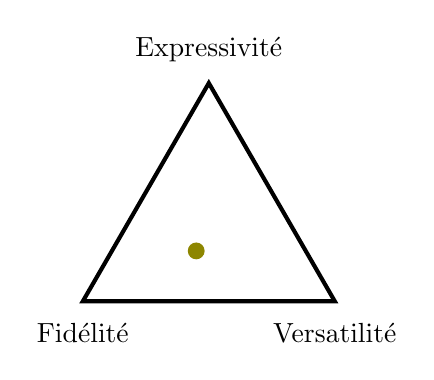
\begin{tikzpicture}[scale=0.8, label distance=1.5mm]
  \coordinate[label=below:Fidélité]  (A) at (0,0);
  \coordinate[label=below:Versatilité] (B) at (4,0);
  \coordinate[label=above:Expressivité] (C) at (2,3.464);
  \draw [line width=1.5pt] (A) -- (B) -- (C) -- cycle;
  \draw [olive, fill=olive, line width=1.5pt] (1.8,.8) circle [radius=.1 cm]; % spec
  \end{tikzpicture}
  Le spectrogramme est à ce jour le compromis le plus apprécié.
}

L'espoir ici est que les erreurs de modélisation des non stationnarités du signal seront négligeables du fait du faible support temporel des fenêtres sur lesquels on applique successivement la tfd. Dans le cas où les fenêtres se recouvrent de moitié, on peut utiliser la transformée en cosinus discret modifiée (tcdm) pour conserver un échantillonnage critique.~\cite{princen1986analysis}

En considérant la tfct, il est alors possible de construire un estimateur \og spectral \fg de la position temporelle de notre dirac :
\begin{equation}
\hat{n}_d = \argmax_t \sum_m X[m, t]
\end{equation}
\`A condition d'utiliser une fenêtre \fg à rampe \og, on peut améliorer la précision temporelle de cet estimateur en réduisant le recouvrement entre fenêtres. La encore, il s'agit d'une amélioration de la précision et non de la résolution. Seule la réduction de l'intervalle d'observation permettra de résoudre la position temporelle de deux diracs proches.

Au travers de ces deux exemples, on voit qu'il est possible d'améliorer dans une certaine mesure la précision des estimations effectuées à partir d'un plan temps / fréquence obtenu grâce à la tfct. Néanmoins, les résolutions temporelles et fréquentielles restent conflictuellement contraintes par la taille de la fenêtre choisie,~\cite{slepian1983some} comme énoncé par le principe d'incertitude d'Heisenberg. On parle ici de variables complémentaires pour le temps et la fréquence, au même titre que la position et la quantité de mouvement en mécanique. Le problème se corse sensiblement lorsque l'on considère des signaux qui possèdent à la fois une localité temporelle et fréquentielle, ce qui est le cas de la plupart des signaux sonores naturels\marginnote[-1cm]{Un exemple iconique étant la note de piano dont la qualité s'exprime autant du côté de la localité temporelle (netteté de l'attaque) que de la localité fréquentielle (pureté des harmoniques).}.

Il paraît alors naturel de considérer des approches à résolution multiples. Tout le problème consiste alors à trouver une représentation qui maximise le potentiel apporté par la multirésolution en terme de fidélité tout en minimisant la perte en expressivité. En effet, la manipulation de données non régulièrement échantillonnées ou recopiées sous divers formats, sont un frein à l'aisance de manipulation.

\marginnote[-3cm]{
   \begin{center}
  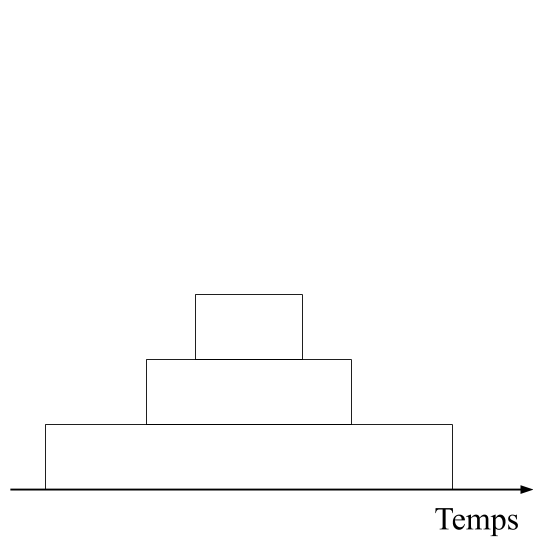
\includegraphics[width=.5\textwidth]{pile}
 \end{center}
Analyses fréquentielles effectuées sur des supports temporels différents.
}

Pour parvenir à une représentation à résolution multiple, l'approche la plus simple conceptuellement consiste à \og empiler \fg plusieurs tfd de largeurs de fenêtre différentes. Cette technique peut se révéler utile dans le cas d'inspection de données ou de prises de décision. Il est par exemple courant de procéder à des fusions ensemblistes de classifieurs d'architectures équivalentes effectuant leurs prédiction à partir de représentations spectrales de résolution différentes. Dans le cas d'un modèle de son, cela induit malheureusement une perte considérable en manipulabilité du fait de la perte d'unicité de la représentation.

Pour éviter cette perte, il est nécessaire de baser notre modèle sur une représentation qui soit à même de partager judicieusement le plan temps / fréquence de manière à mitiger au mieux la contrainte posée par le principe d'incertitude. Un immense travail de la communauté de traitement du signal a été de concevoir ce type de transformée, connue à présent sous le nom de transformée en \og ondelettes \fg.~\cite{mallat1989theory}
\marginnote{
\begin{center}
  % (a) \\
  % 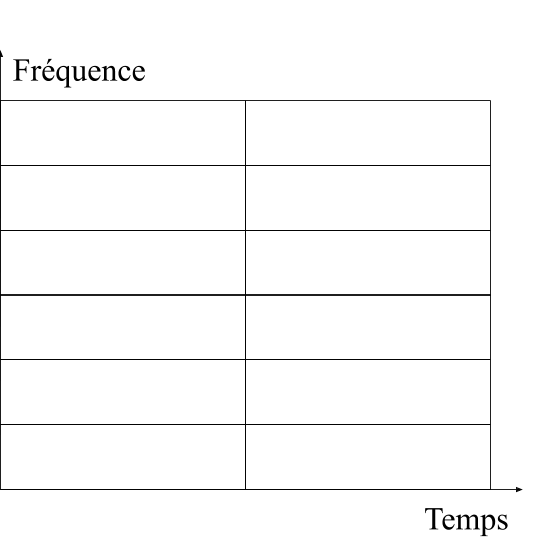
\includegraphics[width=.5\textwidth]{spectrogram.png}
  % (b) \\
  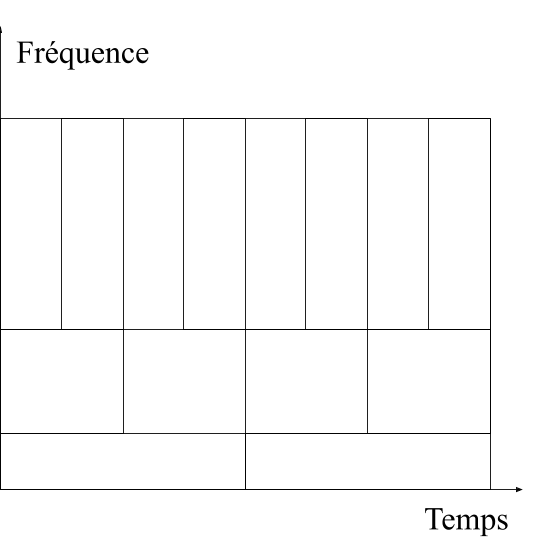
\includegraphics[width=.4\textwidth]{wavelets.png}
\end{center}
Pavage du plan temps / fréquence de la transformée en ondelettes.
}



% Même si les travaux théoriques dans ce domaine ont permis d'ouvrir considérablement les possibilités en terme de conception, je me  tiendrai ici à la forme la plus courante en traitement du signal qui consiste en une construction d'un banc de filtre dyadique à facteur de qualité constant. Ce banc de filtre est constitué d'un ensemble de filtres passe bande à l'octave, \textit{i.e.} la fréquence de coupure supérieure est égale à deux fois la fréquence de coupure inférieure.

Soit ${\psi}(t)$ un filtre de fréquence centrale $\xi$ et de largeur $\xi/Q$, où $Q$ est le facteur de qualité du filtre, un banc de filtre en ondelettes est construit en dilatant
 ${\psi}(t)$ par une séquence géométrique d'échelles $2^{\lambda/Q}$ pour obtenir
\begin{equation}
{\psi_{\lambda}}(t) = 2^{-\lambda/Q} {\psi}(2^{-\lambda/Q} t)\mbox{.}
\end{equation}
La variable $\lambda$ est un facteur d'échelle prenant des valeurs entières entre $0$ et $(J Q - 1)$, où $J$ est le nombre d'octaves couvertes par le banc de filtre.

La transformée en ondelettes d'un signal
${x}(t)$ est obtenue par convolution avec tout les filtres. Un scalogramme, comme celui de la Figure \ref{fig:dirac}, s'obtient par application du module au résultat :
\begin{equation}
{x}(t, \lambda)
= \vert {x} \ast {\psi_{\lambda}} \vert (t)\mbox{.}
\end{equation}


En considérant ce type de décomposition, on obtient alors un pavage du plan temps / fréquence alternatif à celui du spectrogramme. Du fait du principe d'incertitude, les pavés ont la même aire, mais le rapport entre résolution fréquentielle et temporelle est optimalement adapté, contrairement à celui du spectrogramme qui lui reste constant. La Figure \ref{fig:dirac} montre le scalogramme d'une impulsion de Dirac. On y observe clairement l'augmentation de la résolution temporelle en fonction de la fréquence.

\begin{marginfigure}
  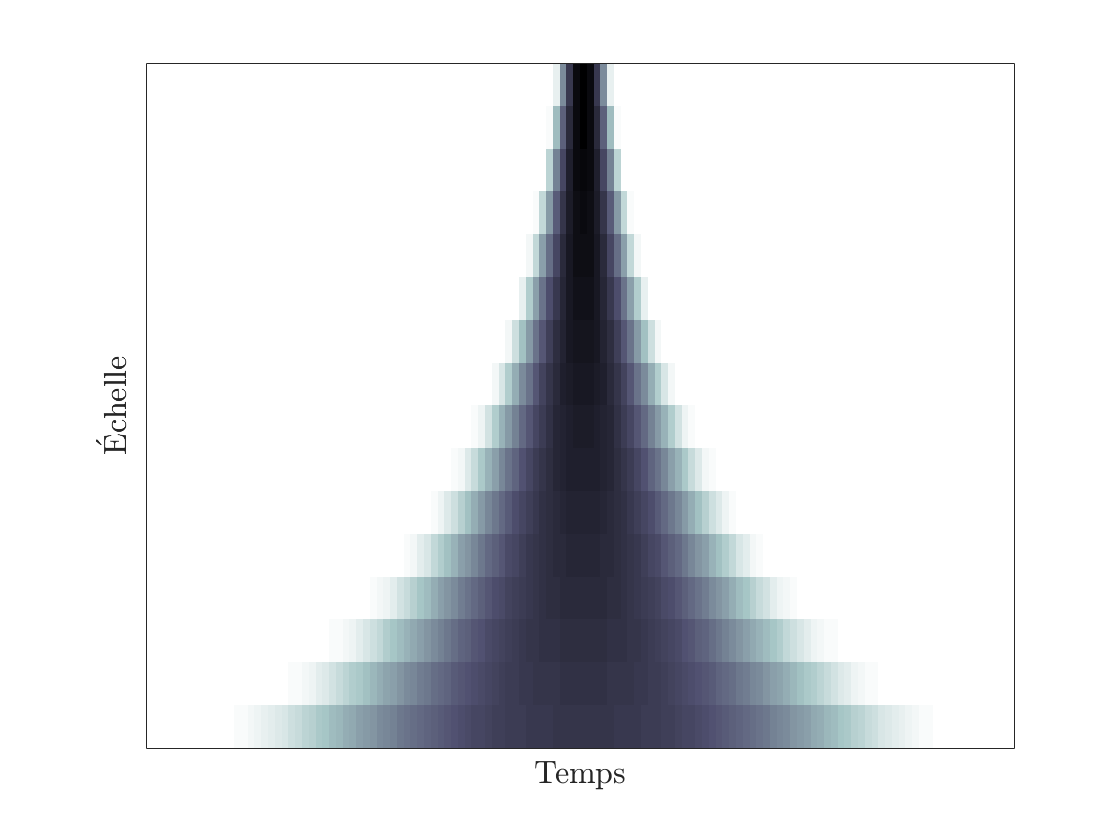
\includegraphics[width=\textwidth]{diracWavelet}
  \caption{Scalogramme d'une impulsion de Dirac.}
  \label{fig:dirac}
\end{marginfigure}

En considérant que le banc de filtre est construit de manière itérative en partant des hautes fréquences, et en notant que le signal observé est d'une durée limitée, une partie du spectre en basse fréquence ne peut être capturé. On ajoute alors un filtre passe bas dit \og de terminaison \fg qui permet de préserver l'unicité de la représentation. Ce dernier filtre, souvent appelé \og fonction d'échelle \fg est peu utilisé dans le cas du traitement de l'audio car il est aisé de capturer le spectre audible avec le banc de filtre en ondelettes et ainsi ne pas considérer les infrasons. Les sorties de ce banc de filtres peuvent être ensuite re-échantillonnées à une fréquence de Nyquist correspondante à la largeur de la bande d'octave du filtre considéré.


Comme le montrent les travaux pionniers effectué par Richard Kronland-Martinet,~\cite{kronland1987analysis} l'application de la transformée en ondelettes paraît avoir d'excellentes propriétés pour le traitement de l'audio, en particulier cette capacité à proposer une analyse multirésolution en préservant la propriété d'unicité.



Quelques décennies plus tard, on doit malheureusement faire le constat que l'utilisation de la transformée en ondelettes reste marginale en traitement de l'audio. Dépasser ce constat arbitraire pour amener des éléments concrets nécessiterait une étude approfondie qui sort du cadre de cet exposé. On peut néanmoins avancer quelques éléments de réflexion.

Une première explication peut être que les fonctions de bases de la transformée en ondelettes, \textit{i.e.} les réponses impulsionnelles des filtres passe bande ont des formes particulièrement irrégulières, non adaptées à l'audio. On peut en effet aisément retenir cet argument pour des ondelettes de Daubechies de faible longueur, mais devient moins recevable pour des longueurs plus élevées, ou pour les ondelettes de Morlet. Cet argument pourrait par contre expliquer pourquoi cette transformée à plutôt pris son essor dans le domaine du traitement d'image, où les discontinuités sont beaucoup plus fortes que pour les signaux sonores. En effet chaque contour d'un objet amène une discontinuité importante dans l'espace couleur, qui, dans le cas de la reconnaissance apporte des éléments d'interprétation très importants, et, dans le cas du codage, se doit d'être représenté en détail, sous peine d'engendrer des artéfacts de type \og lissage \fg très pénalisants.

Une seconde explication, finalement peut être plus déterminante, peut avoir trait à la faible expressivité de la transformée. L'interprétation  du spectrogramme est intuitive et permet une manipulation fine du contenu spectral d'un signal audio par exemple pour des opérations de masquage présentées dans la section dédiée à l'\lnameref{sec:asa}. L'échantillonnage non régulier en temps et en fréquence de la transformée en ondelettes ne simplifie pas l'expression des transformations que l'on souhaite généralement opérer (transposition, étirement, ...). La version filtrée pour obtenir un échantillonnage régulier en temps est plus appropriée, mais au prix de la perte de toute notion de multirésolution.

\marginnote[-2cm]{
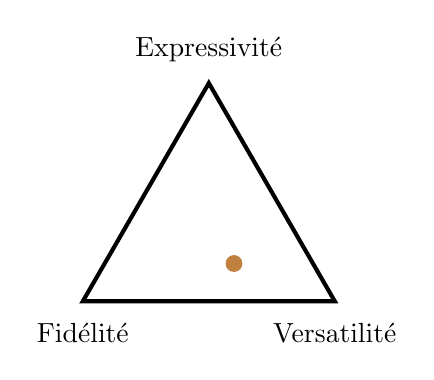
\begin{tikzpicture}[scale=0.8, label distance=1.5mm]
  \coordinate[label=below:Fidélité]  (A) at (0,0);
  \coordinate[label=below:Versatilité] (B) at (4,0);
  \coordinate[label=above:Expressivité] (C) at (2,3.464);
  \draw [line width=1.5pt] (A) -- (B) -- (C) -- cycle;
  \draw [brown, fill=brown, line width=1.5pt] (2.4,.6) circle [radius=.1 cm]; % wavelets
  \end{tikzpicture}
  La transformée en ondelettes est en théorie assez versatile grâce à la multirésolution, mais peu de travaux démontrent son expressivité.
}

\marginnote[-4cm]{
   \begin{center}
  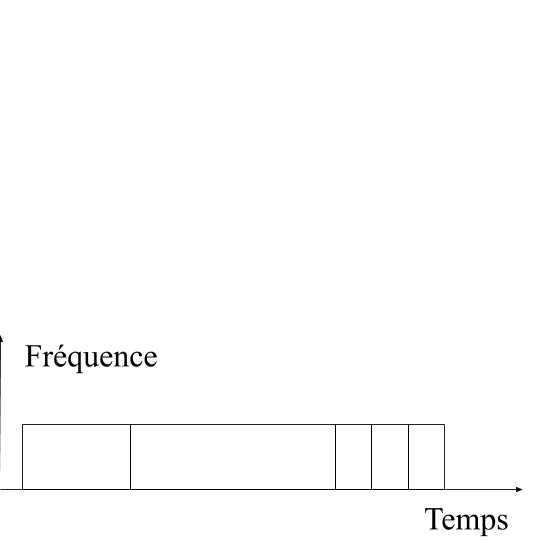
\includegraphics[width=.5\textwidth]{seq}
 \end{center}
Analyses fréquentielles effectuées sur des support temporels différents séquencées dans le temps.
}


En tout état de cause, dans le domaine de l'audio, la grande majorité des systèmes de traitement considère une représentation de type tfct, avec des paramètres de résolution et de précision constants, adaptés à la tâche. Dans les applications de codage, on trouve des mécanismes à résolution multiple de type alterné, implantés grâce des tcdm à plusieurs largeurs de support.~\cite{brandenburg1999mp3} Au sein du codeur, une heuristique détermine parmi les résolutions possibles, la résolution la plus adaptée au vu du signal contenu dans l'intervalle d'observation considéré. Cet échantillonnage non régulier de l'axe temporel permet une meilleure fidélité et flexibilité si l'heuristique est adaptée, ceci au détriment de l'expressivité, le plan temps / fréquence induit étant non régulier, ce qui n'est généralement pas un facteur limitant dans des chaînes de codage.

On considère donc ici que dans l'intervalle d'observation, une source sonore est dominante et que la source est structurée soit de manière temporelle soit de manière fréquentielle. Dans le cas d'un contenu polyphonique avec une structure à la fois en temps et en fréquence, cette approche se révèle bien entendu inopérante. La définition d'une méthode d'analyse/synthèse multirésolution reste donc, avec les éléments présentés ici, un champ de recherche encore largement ouvert.

\section{ \nmu Sinusoïdes à court terme}  \label{sec:sct}

Lorsque l'on observe le spectrogramme d'un instrument de musique tonal, comme celui d'une note de piano, il apparaît clairement que l'énergie est concentrée en un ensemble réduit de zones fréquentielles. On dit que ces signaux sont parcimonieux en fréquence. C'est, dans une certaine mesure, le cas de la parole. Comme le montrent les exemples de "sine-wave speech", un nombre réduit de sinusoïdes judicieusement placées aux zones de résonances formantiques suffisent à rendre le signal intelligible.\marginnote[-2cm]{
\begin{center}
  \fbox{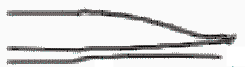
\includegraphics[width=.4\textwidth]{Fig23.png}}
\end{center}
 Un exemple de ce type de synthèse de parole est disponible pour écoute : \url{http://webpages.mcgill.ca/staff/Group2/abregm1/web/snd/Track23.mp3}.}

En suivant cette observation, on peut modéliser chaque zone de forte énergie du plan temps / fréquence par une composante sinusoïdale à court terme. Pour cela, il est commun d'identifier des maxima locaux dans chaque spectre du spectrogramme pour identifier un ensemble de \og pics spectraux \fg, ou \og atomes \fg temps / fréquence. On obtient alors le modèle de son suivant :
\begin{equation}
  x[n] = \sum_{c=1}^{C_t} a_{t, c} \mathrm{sin}(2 \pi f_{t, c} n + \phi_{t, c})
  \label{eq:sct}
\end{equation}
où $t$ et $c$ désignent respectivement l'indice temporel de trame et l'indice de composante dans cette trame et $C_t$ désigne le nombre de composantes par trame $t$.

Les paramètres de fréquence $f_{t, c}$, d'amplitude $a_{t, c}$, et de phase $\phi_{t, c}$ de chaque atome $p_{t, c}$ peuvent être estimés grâce aux techniques évoquées dans la section précédente, qui se basent sur le spectrogramme. On voit par exemple sur la Figure \ref{fig:ct} l'impact de l'augmentation de la taille de fenêtre de la tfct utilisée pour identifier les composantes à court terme. Dans le cas de signaux polyphoniques, on voit qu'il peut être ardu de préserver un bon compromis résolution temporelle / résolution fréquentielle.

\begin{figure*}[t]
  \footnotesize
  \begin{tabular}{ccc}
    (a) & (b) & (c)  \\
  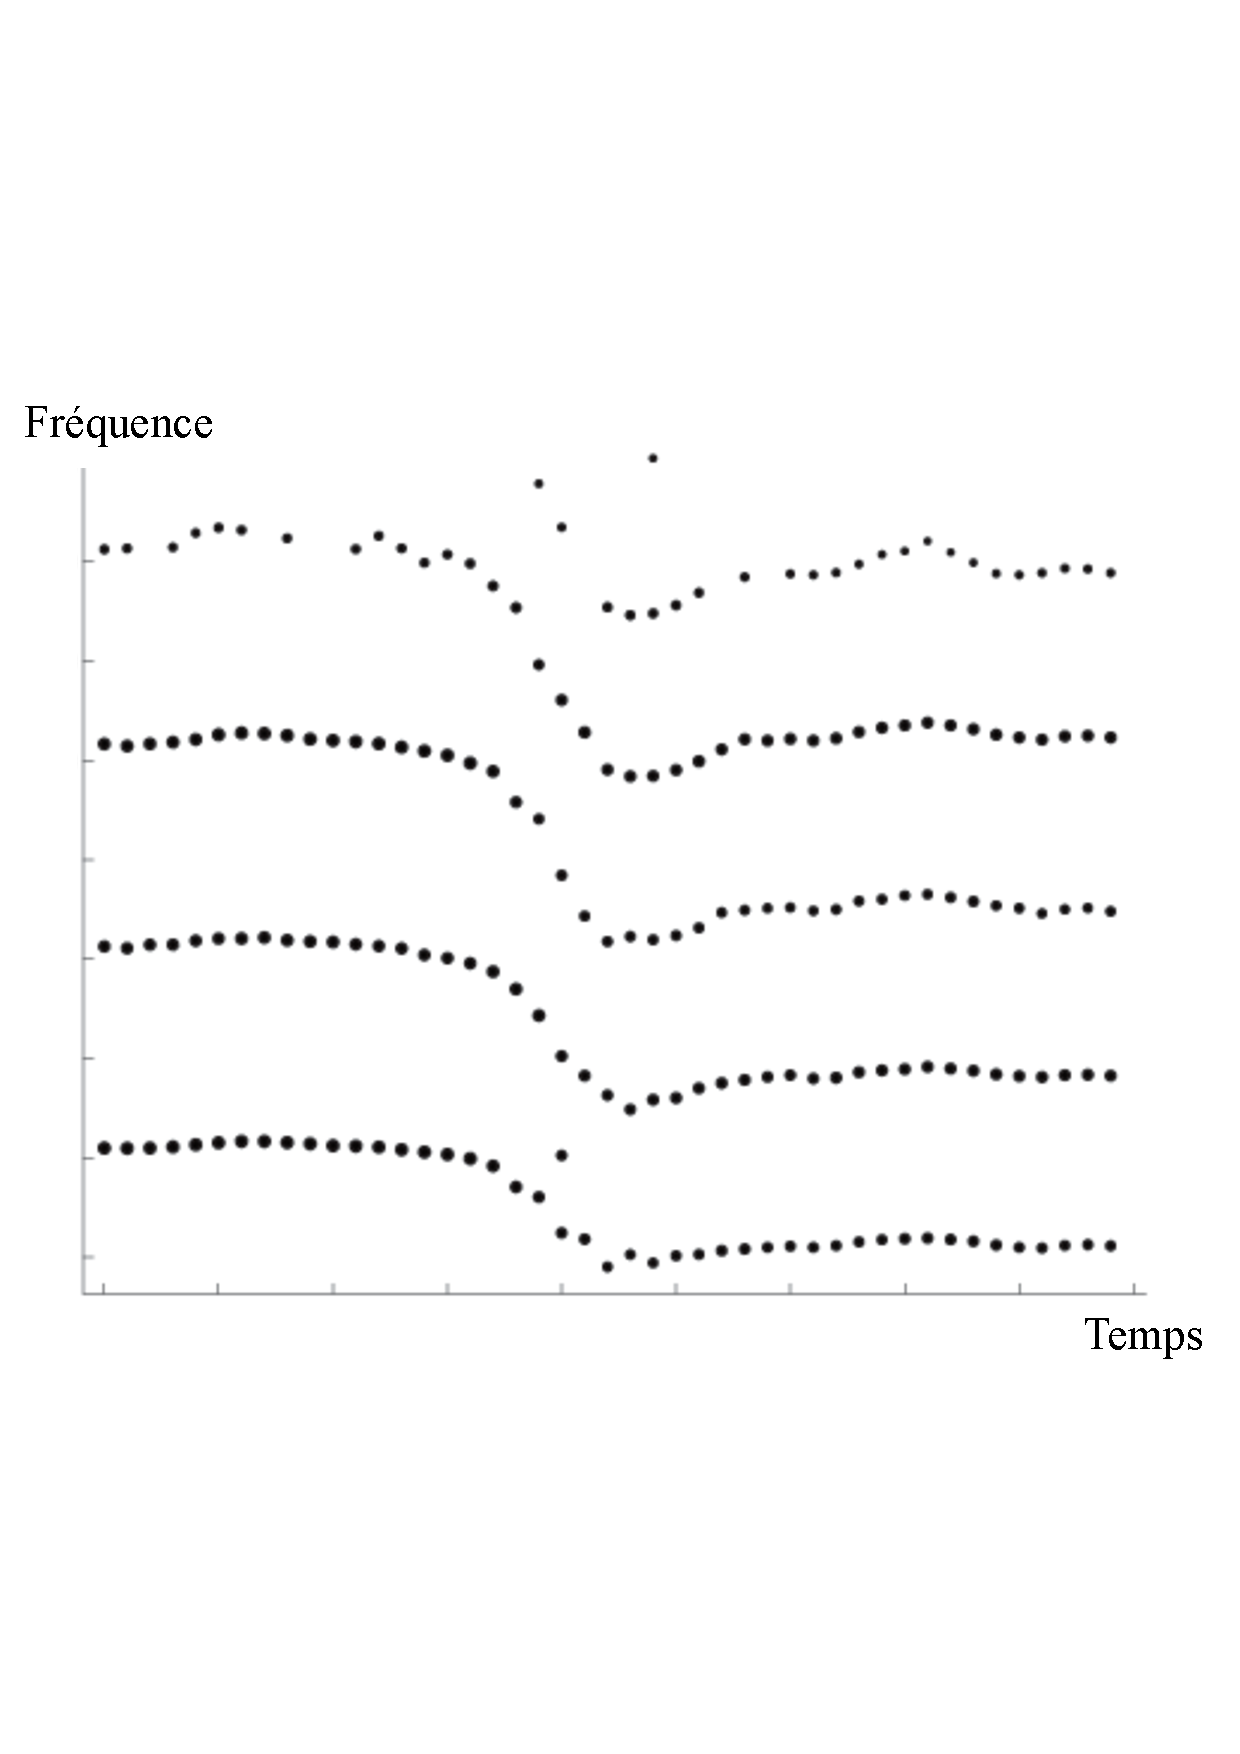
\includegraphics[width=.3\textwidth]{voice_1024_512xp} &
  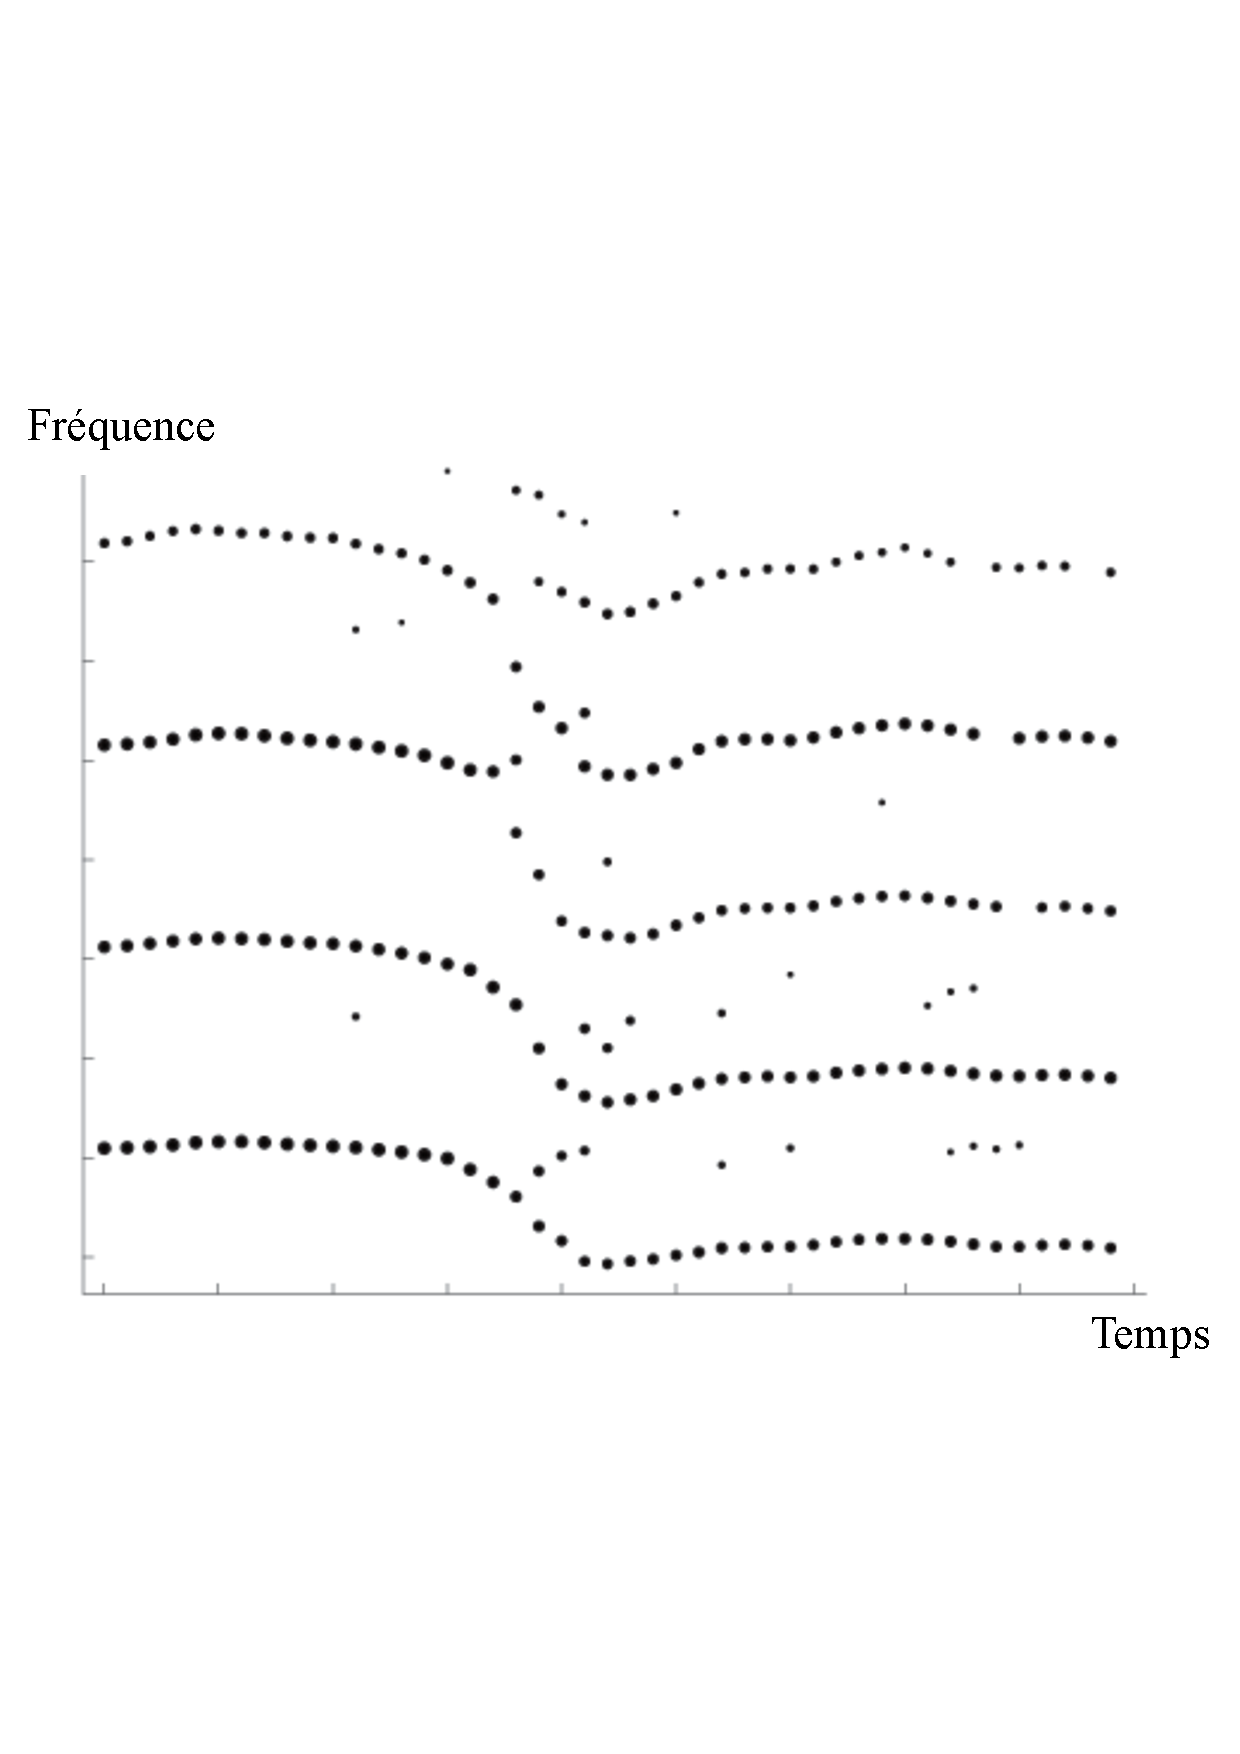
\includegraphics[width=.3\textwidth]{voice_2048_512xp} &
  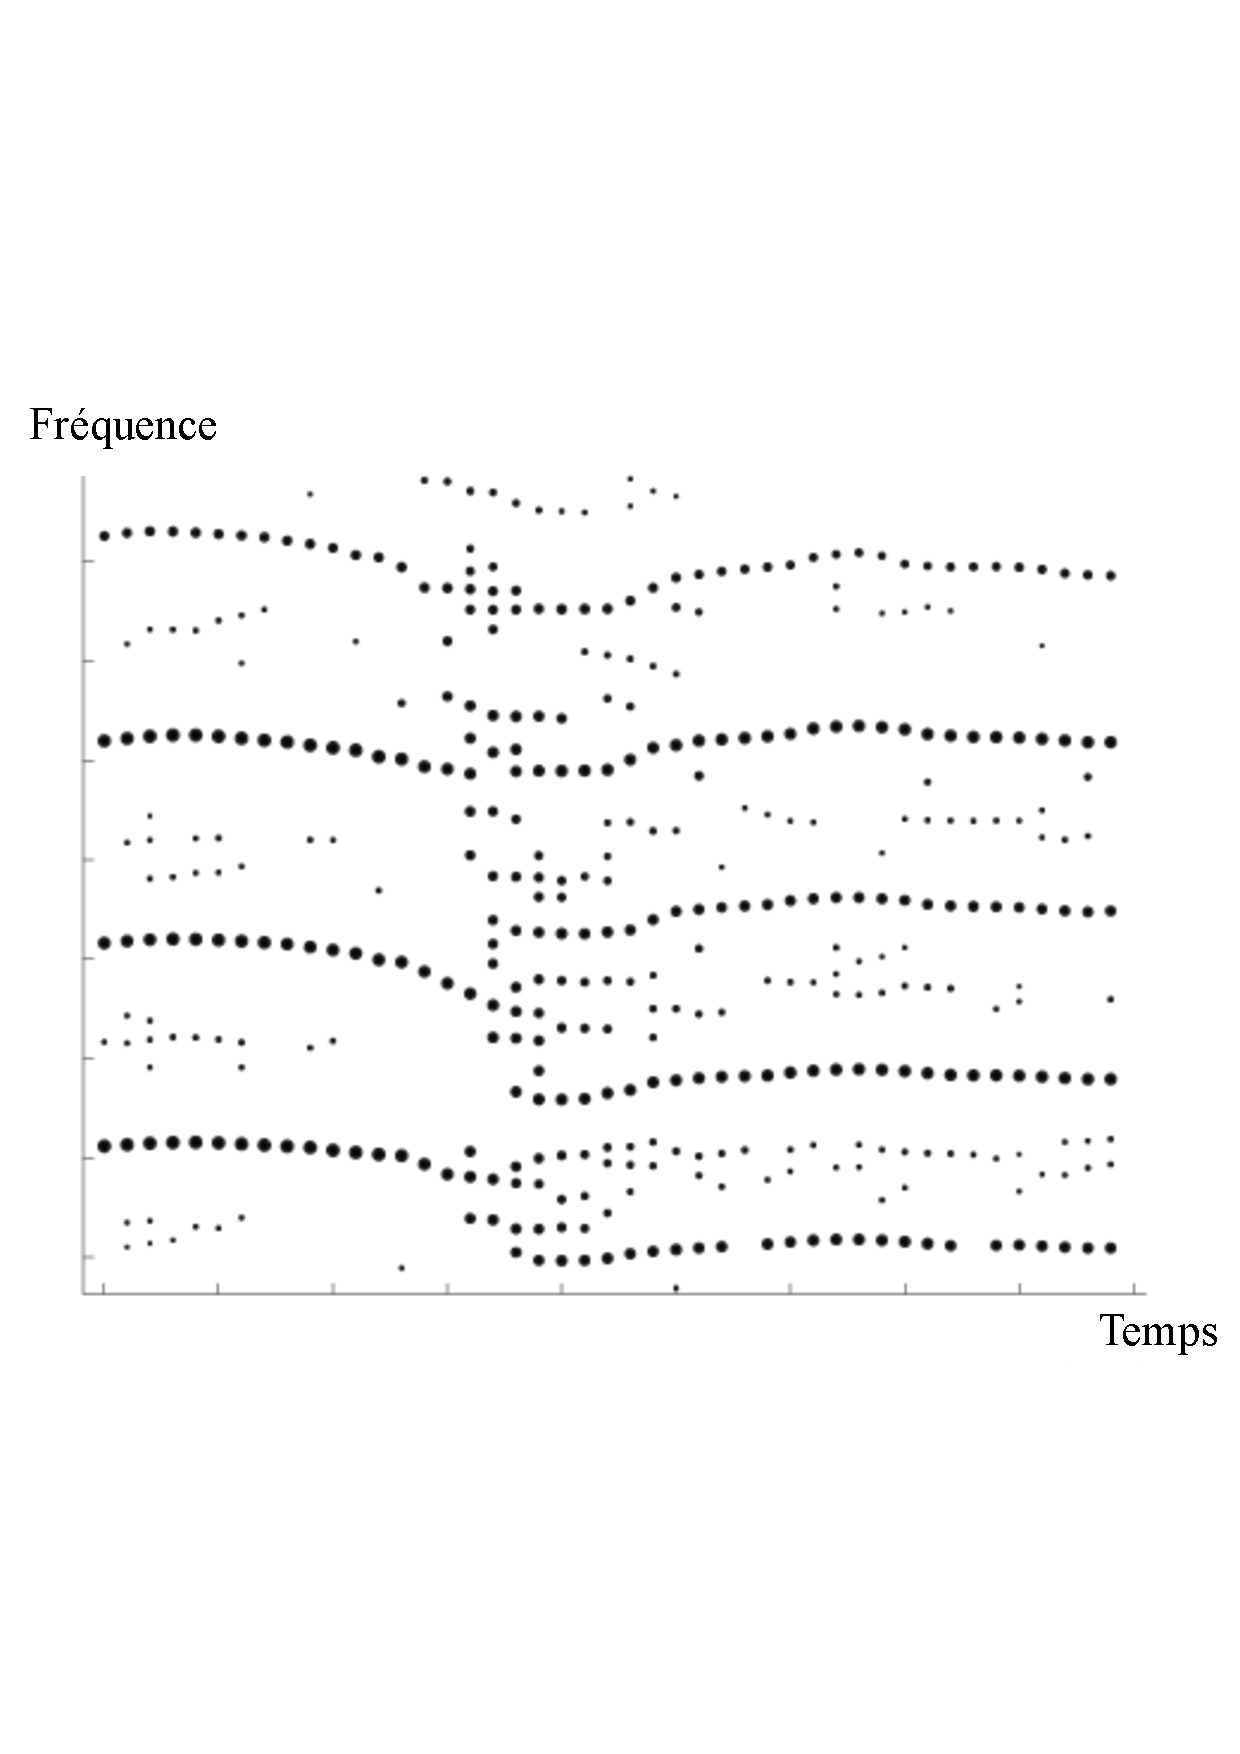
\includegraphics[width=.3\textwidth]{voice_4096_512xp} \\
\end{tabular}
  \caption{Influence de la taille de fenêtre de la tfct utilisée pour estimer un modèle sinusoïdal à court terme d'un glissando de trombone. De gauche à droite, la taille est de 25 (a), 50 (b), et 100 ms (c), pour un pas d'avancement de 10 ms. Chaque point correspond  à une composante à court terme $p_{t, c}$ et sa taille est fonction de l'amplitude de la composante $a_{t, c}$.}
  \label{fig:ct}
\end{figure*}

L'effectivité du modèle sinusoïdal à court terme est motivée par la parcimonie des signaux sonores. Elle se révèle néanmoins très robuste à la réduction de cette dernière pour peu que le nombre de composantes soit suffisant. En effet, l'expansion de Karhunen-Lo\`eve de signaux bruités montre qu'une représentation sinusoïdale de ce type de signaux est valide, à condition que les atomes soient suffisamment nombreux et de fréquences suffisamment proches pour que la densité spectrale de puissance dans ces zones varie lentement dans le temps. Le nombre de composantes par intervalle de temps $C_t$ est donc un facteur déterminant. En pratique, dans un compromis favorisant la fidélité et la versatilité au détriment de l'expressivité, on choisira $C_t$ en fonction de contraintes de complexité, \textit{i.e.} le plus grand nombre possible.

%La précision de ces estimations peut être améliorer par des techniques de sur échantillonage en fréquence et en temps, au détriment du coût de calcul. Ceci étant dit, les limites de cette technique sont bien illustrés dans la figure suivante :

% voice_1024_512.eps

% Ce problème d'estimation dépassant largement la problématique de la modélisation du signal audio, un effort conséquent d'amélioration des ces estimateurs a été effectué par la communauté de traitement du signal. Les approches les plus efficaces et les plus élégantes pour ce faire se basent sur des relations entre les paramètres spectraux de plusieurs transformées de Fourier effectuées après différents traitements du signal observé. La technique du reassignement spectral~\cite{auger1995improving} considère le rapport entre la DFT du signal fenêtré et la DFT du signal fenêtré par la dérivée de la fenêtre :
% \begin{equation}
% t
% \end{equation}
% En considérant le rapport de la DFT du signal et celle de la DFT de la dérivée du signal, on obtient une autre série d'estimateurs. On a prouvé l'équivalence théorique de ces dernières à la technique du réassignement, supportée par des expérimentations montrant des performances similaires~\cite{lagrangeJaes07}.

Dans un objectif d'expressivité, il est à contrario important que l'observation  soit en adéquation avec le modèle utilisé, c'est-à-dire que les composantes sinusoïdales modélisent effectivement des composantes quasi-périodiques présentes dans le signal analysé. En effet, même si une partie bruitée du signal peut être raisonnablement modélisée avec des composantes sinusoïdales de fréquence proches et de phase arbitraire, il sera difficile avec cette modélisation de préserver une bonne qualité d'écoute lors de la manipulation de ce modèle, par exemple pour effectuer un étirement ou une transposition.

Il convient donc d'être à même de sélectionner parmi les composantes candidates, celles qui sont les plus appropriées en fonction de critères dits de \og sinusoïdalité \fg. Une manière de faire consiste à corréler, pour chaque pic candidat, sa réponse fréquentielle à celle du spectre d'une sinusoïde dont les paramètres sont résultant du processus d'estimation.~\cite{peak-selection} Le degré de corrélation permet alors de quantifier la pertinence du modèle vis-à-vis de l'observation. Une étude comparative semble montrer l'intérêt de cette approche.~\cite{wells2010comparative} Dans cet algorithme, les références au modèle sont construites dynamiquement mais peuvent aussi être échantillonnées. On se rapproche alors du principe des algorithmes de poursuite de sous espaces.

Le principe de ces algorithmes est de s'affranchir des contraintes de la base de Fourier en disposant d'un (très) large dictionnaire d'atomes redondants et de déterminer la combinaison optimale de ces atomes permettant de réduire l'erreur d'approximation. Dans de la modélisation de données audio-numériques, ces atomes sont typiquement des sinusoïdes tronquées ou fenêtrées. L'algorithme "matching pursuit" (mp) proposé par Stéphane Mallat~\cite{mallat1993matching} permet de résoudre efficacement ce problème en considérant un algorithme glouton, où l'atome mis à l'échelle ayant la meilleure corrélation avec le signal résiduel (égal au signal d'origine au début de l'algorithme) est itérativement sélectionné puis soustrait. L'application de cet algorithme à des signaux musicaux peut poser des problèmes, dont certains ont été étudiés par Rémi Gribonval.~\cite{gribonval1996sound} %Par exemple, dans le cas de signaux non stationnaire en amplitude, continuitél'algorithme aura tendance à construire des approximations non satisfaisantes.

La Figure \ref{fig:gribonval} illustre deux cas typiques de non stationnarités rencontrées dans les signaux musicaux. Le premier consiste en une composante sinusoïdale dont l'amplitude est modulée de manière sinusoïdale, Figure \ref{fig:gribonval}(a). C'est une modulation typique d'un tremolo. Le second consiste en une composante sinusoïdale dont l'amplitude est modulée par la multiplication d'une marche d'escalier et d'une exponentielle décroissante, Figure \ref{fig:gribonval}(b). C'est une modulation typique d'une corde frappée ou pincée comme le piano ou le clavecin.


\begin{marginfigure}
  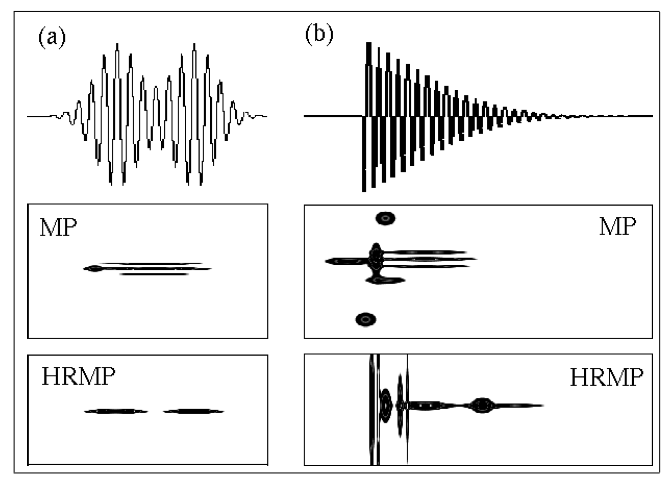
\includegraphics[width=\textwidth]{gribonval.png}
  \caption{Deux composantes sinusoïdales dont l'amplitude est modulée a) sinusoïdalement, b) exponentiellement et décompositions correspondantes par deux algorithmes de poursuite (mp et hrmp). Figure issue de la référence \no 48.}
  \label{fig:gribonval}
\end{marginfigure}

Dans le premier cas, l'algorithme mp identifie d'abord une composante avec un support temporel couvrant l'intégralité du signal. Deux autres composantes viennent ensuite annuler certaines parties de cette première. Dans le second cas, le changement abrupt d'énergie étant difficilement modélisable aves les fonctions de base à disposition, de nombreuses composantes d'annulation sont nécessaires, amenant à un effet de pré écho, l'énergie ajoutée n'étant que partiellement enlevée. Pour pallier ces problèmes, des contraintes de non négativité ont été proposées pour améliorer l'algorithme de poursuite, alternative nommée "high resolution matching pursuit" (hrmp). En réduisant les contributions destructives, \textit{i.e.} des atomes sélectionnés pour se soustrairent à des contributions résiduelles d'atomes précédemment sélectionnés, cette approche est plus efficace au sens où l'énergie globale des atomes (somme des enveloppes des atomes utilisés) est plus faible. Dans des approches codage, le fait d'utiliser un nombre de composantes réduit est désirable pour des raisons de contrôle du débit. Cette propriété est, dans une certaine mesure, souhaitable également pour des applications de manipulation car cela permet d'avoir un nombre de paramètres réduit à manipuler. Il est par contre important que le gain en compacité ne se fasse au détriment de l'expressivité.


\marginnote[0cm]{
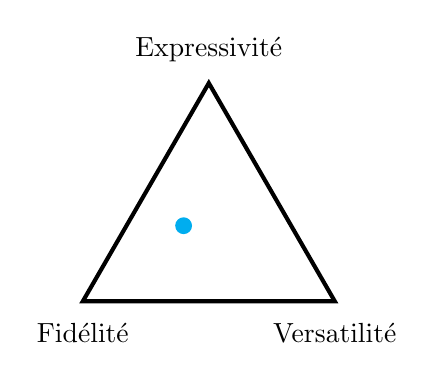
\begin{tikzpicture}[scale=0.8, label distance=1.5mm]
    \coordinate[label=below:Fidélité]  (A) at (0,0);
    \coordinate[label=below:Versatilité] (B) at (4,0);
    \coordinate[label=above:Expressivité] (C) at (2,3.464);
    \draw [line width=1.5pt] (A) -- (B) -- (C) -- cycle;
    \draw [cyan, fill=cyan, line width=1.5pt] (1.6,1.2) circle [radius=.1 cm]; % sct
  \end{tikzpicture}
  Les modèles sinusoïdaux à court terme sont des modèles de son avec une expressivité améliorée par rapport au spectrogramme au prix d'une perte relative en fidélité et versatilité.
}

De manière générale, il est difficile de critiquer les approches basées poursuite dans le sens où leur pertinence vis-à-vis de la tâche va grandement dépendre du dictionnaire choisi. On notera tout de même que ces approches sont construites avec un objectif d'approximation et non d'identification. Par exemple dans le cas de la sinusoïde modulée de manière sinusoïdale, Figure \ref{fig:gribonval}(a), les deux algorithmes de poursuites sont tout deux à même de fournir une bonne approximation du signal, mais \og n'identifient \fg pas le phénomène, le dictionnaire n'ayant pas ce type de forme à disposition. Dans une application de type codage, on préfèrera sans doute la seconde approximation pour des raisons d'efficacité de la représentation. Pour ce qui est de la notion d'expressivité, le choix entre les deux modèles seront une affaire de compromis en fonction du type de manipulation souhaité. On se trouve donc avec un compromis de modèle favorisant la fidélité et la versatilité, au détriment de l'expressivité. Il est en effet difficile de déterminer des fonctions simples de manipulation dans le cas d'un dictionnaire très largement redondant.

%Ces approches, comme la transformée en ondelettes, ont trouvés application plutôt dans le domaine du traitement de l'image, où le caractère hautement non stationnaire des transitions entre objets sont très mal approximé par des fonctions régulières comme celle de Fourier.

\section{ \nmu Sinusoïdes à long terme}  \label{sec:slt}

L'approche sinusoïdale à court terme effectue des observations discrètes d'un processus de production sonore qui est par essence continu. Dans le cas de nombreux instruments de musique, il est raisonnable de considérer que ce processus continu peut être représenté par une somme de sinusoïdes dont les paramètres varient \textsl{lentement} dans le temps. Une variation lente s'entend ici de l'ordre de la dizaine de Hertz. Dans ce cas, le modèle sinusoïdal à long terme est particulièrement à propos. Ce modèle peut s'écrire comme suit :
\begin{equation}
x[n]=\sum_{l=1}^{L} a_{l}[n] \sin \left(\frac{2 \pi}{F_{s}} f_{l}[n] \cdot n + \Phi_k \right)
\label{eq:slt}
\end{equation}
où $a_{l}[n]$ et $f_{l}[n]$ sont des signaux contrôlant respectivement l'amplitude et la phase des $L$ oscillateurs composant le modèle. Au contraire du modèle court terme de l'équation \ref{eq:sct}, il est donc possible de modéliser des signaux non stationnaires et s'avère donc pertinent pour modéliser des signaux à long terme.

Chaque composante sinusoïdale est souvent appelée \textsl{partiel} pour des raisons historiques. En effet, ce modèle a été appliqué originellement à des sources monophoniques, dont les composantes périodiques étaient appelées partiels, l'ensemble des partiels composant la note. Dans le cas de signaux harmoniques, les partiels sont également souvent appelées harmoniques et la première harmonique, l'harmonique fondamentale.


\marginnote[0cm]{
\begin{center}
  \scalebox{1}{
  % \documentclass[tikz,border=10pt]{standalone}
% \usepackage{tikz,pgf}
% \usetikzlibrary{positioning,shapes,shadows,arrows}
%
% \begin{document}
\begin{tikzpicture}[
nonterminal/.append style={join=by ->},
tip/.style={->,shorten >=1pt},every join/.style={rounded corners},
terminal/.style={
% The shape:
rectangle,minimum size=6mm,rounded corners=1mm,
% The rest
very thick,draw=black!50,
top color=white,bottom color=black!10,
font=\ttfamily},
point/.style={circle,fill=black,minimum size=2pt},
%every node/.style=draw,
line/.style ={draw, thick, -latex',shorten
  >=2pt}]
%%%%%%%%%%%%%%%%%%%%%%%%%%%%%%%%%%%%%%%%%%%%%%%%%%%%%%%%%%%



\matrix [column sep=10mm,row sep=5mm]
{
\node (i1) {}; \\
\node [terminal] (i2) {tfct}; \\
\node [terminal] (i3) {sélection de pics}; \\
\node [terminal] (i4) {suivi de partiel}; \\
\node  (i5) {}; \\
};

\begin{scope}[every path/.style=line]
  \path (i1) -- node [right] {signal} (i2);
  \path (i2) -- node [right] {spectrogramme} (i3);
  \path (i3) -- node [right] {atomes } (i4);
  \path (i4) -- node [right] {partiels} (i5);
\end{scope}

\end{tikzpicture}
% \end{document}
}
\end{center}

Schéma fonctionnel des approches d'identification de composantes long terme (les partiels) par restauration de continuité. Le signal sonore est projeté sur le plan temps / fréquence où des atomes court terme $p_{t, c}$ correspondant à des maxima locaux sont identifiés. Certains atomes de trames successives et de fréquence proche formeront des partiels $\mathcal{P}_{p}$.
}

Ce modèle est particulièrement expressif car il permet des modifications du signal d'intérêt comme la translation, la transposition, ou encore l'étirement, simplement en manipulant les paramètres des partiels. Ces transformations sont de plus de faible coût car les paramètres sont échantillonnés à une fréquence environ 1000 fois plus faible que le signal audio-numérique. Le processus de synthèse est également aisé à mettre en \oe{}uvre avec les moyens computationels actuels. Dans le cas d'un très grand nombre de composantes, des algorithmes d'élagages perceptuels~\cite{lagrangeDafx01} peuvent être mis en place. L'étape d'analyse, \textit{i.e.} l'estimation des paramètres à partir d'un signal sonore est par contre, particulièrement ardue dans le cas général.

Dans notre présentation des algorithmes d'estimation des paramètres long terme, on supposera que le signal analysé est composé d'une ou plusieurs sources dont une grande partie de l'énergie peut être correctement approximée par ce modèle. On fera état ici des approches dites de suivi de partiels, dont le but est de \og restaurer \fg la continuité temporelle entre les composantes à court terme d'un même partiel. Le résultat de cette étape de continuation est une version échantillonnée des paramètres de contrôle nécessaire au modèle de l'équation \ref{eq:slt} :
\begin{equation}
\mathcal{P}_{p}=\left(\mathcal{P}_{p}[t]\right)_{t \in\left[b_{p}, \cdots, b_{p}+l_{p}-1\right]}
\end{equation}
où $t$ est l'indice de trame du spectrogramme, $b_{p}$ est l'indice de trame de début du partiel, et $l_{p}$ le nombre de trame où le partiel est actif. Chaque composante court terme se décrit comme suit :
\begin{equation}
\mathcal{P}_{p}[t]=\left(n, \phi_{p}[t], a_{p}[t], f_{p}[t]\right)
\end{equation}
Le passage de cette version échantillonnée à court terme des paramètres à l'échantillonnage signal peut se faire par différentes techniques d'interpolation.

Dans l'article fondateur de George Mc Aulay,~\cite{mcaulay} il est proposé \og d'identifier \fg ces partiels en reliant entre eux des atomes de trames successives. L'algorithme proposé est itératif. Supposant un ensemble de partiels identifié à la trame $t$, on va chercher à prolonger ces partiels à la trame $t+1$ en commençant par le partiel de plus basse fréquence, tel que la différence entre la fréquence du partiel $\mathcal{P}_{p}$ à la trame $t$ et la fréquence d'un atome disponible à la trame $t+1$ est minimale :
\begin{equation}
c_{\mathrm{min}} = \argmin_{c}\left|f_{t+1, c}-f_{p}[t]\right|
\label{eq:mac}
\end{equation}
Si cette continuation n'engendre pas un saut en fréquence trop conséquent :
\begin{equation}
\left|f_{t+1, c_{\mathrm{min}}}-f_{p}[t]\right|<\Delta_{f}
\label{eq:macseuil}
\end{equation}
où le seuil en fréquence $\Delta_{f}$ est un paramètre du modèle, alors le partiel $\mathcal{P}_{p}$ est prolongé à trame $t+1$. Dans un principe d'allocation exclusif, l'atome $p_{t+1, c_{\mathrm{min}}}$ ne pourra pas être utilisé pour la continuation d'un autre partiel. Chaque atome non utilisé à la trame $t+1$ devient alors un partiel qui sera potentiellement prolongé aves des atomes de la trame $t+2$.

On constate ici que la structure de données se complexifie sensiblement par rapport à la plupart de celles introduites avec des outils de traitement du signal canoniques, amenant une approche plus \og informatique \fg à une problématique de traitement du signal. Cette modélisation plus riche a permis une flexibilité de manipulation qui a donné lieu à la proposition d'un large ensemble d'heuristiques qui ne seront pas présentées ici, même si elles ont leur intérêt pour la qualité du rendu sonore de ce type d'approche.


\marginnote[-2.5cm]{
  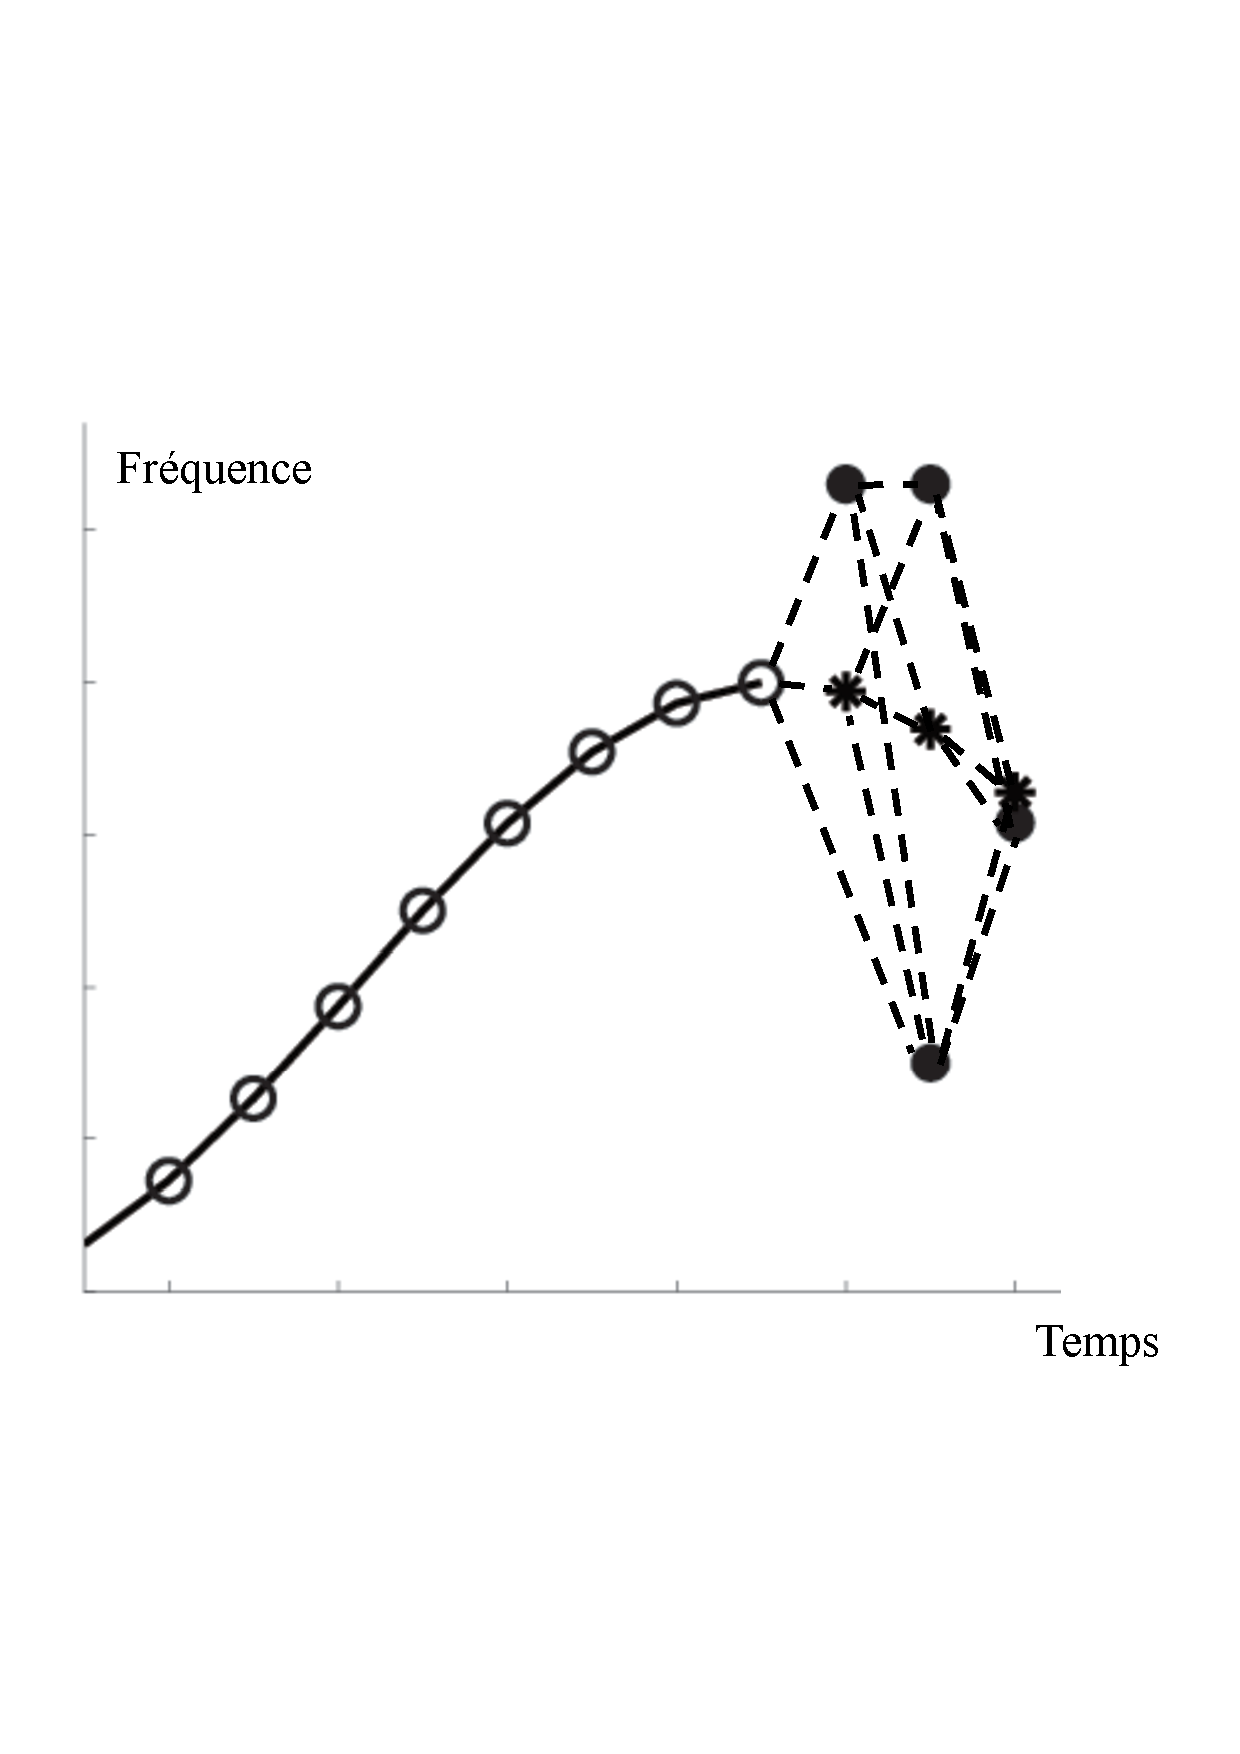
\includegraphics[width=.5\textwidth]{trackingxp2xp2}

Une étape de continuation du partiel $\mathcal{P}_{p}$ dans les trames d'indices $t+1$ à $t+l$. La sélection de la meilleure continuation se fait parmi les continuations (traits pointillés) composées des atomes  (point noirs) $p_{t+1...l, c}$ de fréquence $f_{t+1...l, c}$ proches des valeurs de fréquence prédites $\hat{f}_{p}[t+1...l]$ obtenue par prédiction linéaire (étoiles) et ces valeurs prédites.}

La contrainte exprimée par l'équation \ref{eq:macseuil} revient à avoir un prédicteur constant en fréquence. Dans le cas d'un modèle court terme de bonne qualité, par exemple dans le cas d'un signal monophonique à structure harmonique comme une note de flûte, cette heuristique peut être raisonnable. Dans le cas de signaux non stationnaires comme le glissando de trombone de la Figure \ref{fig:ct}, de signaux bruités et / ou polyphoniques, il est utile d'améliorer la finesse du prédicteur en considérant un prédicteur linéaire appliqué aux séries temporelles des paramètres long terme. Le faible échantillonnage de ces séries temporelles nécessite des estimateurs adaptés comme celui de Burg.~\cite{burg1968new}

Dans ce cas, à partir des fréquences du partiel de la trame $t-g$ à la trame $t$ où $g$ est la longueur de la série temporelle des fréquences pris en compte, on obtient par application du prédicteur linéaire une prédiction des valeurs des fréquences du partiel pour les trames suivantes : $\hat{f}_{p}[t+1...l]$, où $l$ est l'horizon temporel utilisé.

La contrainte d'évolution lente des paramètres dans un modèle d'évolution quasi stationnaire se traduit naturellement par un seuil sur le delta de fréquence, voir Equation \ref{eq:macseuil}. Dans le cas d'un modèle non stationnaire des paramètres long terme, on trouve un gain à considérer une analyse spectrale de ces évolutions possibles pour mieux déterminer les continuations à effectuer. Pour ce faire, parmi toutes les continuations possibles, la continuation qui engendre le moins de hautes fréquences est privilégiée. Là encore, du fait du faible échantillonnage des paramètres, des outils d'estimation spectrale spécifiques sont nécessaires.

Soit un partiel $\mathcal{P}_{p}$ que l'on cherche à prolonger dans les trames d'indices $t+1$ à $t+l$. On dispose des prédictions des valeurs de fréquence dans ces trames : $\hat{f}_{p}[t+1...l]$. Les atomes $p_{t+1...l, c}$ proches de ces prédictions sont sélectionnés. Toutes les successions de valeurs de fréquences sont alors considéré comme des signaux et analysé spectralement. La continuation engendrant le moins de contenu haute fréquence est sélectionné.


Les bons résultats en terme de rendu sonore obtenu par cette chaîne d'analyse dans le cas  de la modélisation long terme sous contrainte de débit~\cite{lagrangeTaslp06} et l'interpolation de données manquantes,~\cite{lagrangeJaes05} montrent l'intérêt de la modélisation des modulations long terme, au moins du point de vue perceptif.

Fort de cette observation, Martin Raspaud a étudié un modèle long terme hiérarchique qui permet des manipulations riche comme par exemple de l'étirement temporel de notes vibrées.~\cite{raspaud2007modeles} Le principe est de considérer les paramètres long terme comme des signaux, eux mêmes modélisables comme des sinusoïdes dont les paramètres évoluent, cette fois ci, très lentement en fonction du temps. Il est alors aisé de contrôler les modulations de haut niveau comme le vibrato ou le tremolo.


\marginnote[0cm]{
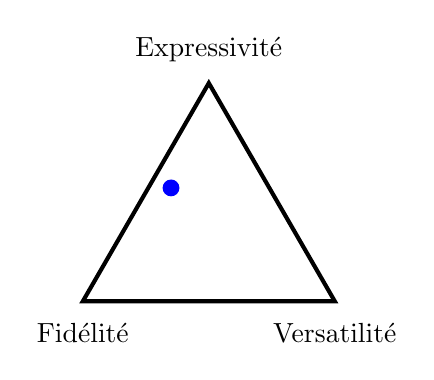
\begin{tikzpicture}[scale=0.8, label distance=1.5mm]
  \coordinate[label=below:Fidélité]  (A) at (0,0);
  \coordinate[label=below:Versatilité] (B) at (4,0);
  \coordinate[label=above:Expressivité] (C) at (2,3.464);
  \draw [line width=1.5pt] (A) -- (B) -- (C) -- cycle;
  \draw [blue, fill=blue, line width=1.5pt] (1.4,1.8) circle [radius=.1 cm]; % slt
  \end{tikzpicture}
  Le modèle sinusoïdal à long terme est expressif et fidèle, mais pour un champ réduit de signaux sonores.
}


D'une grande élégance formelle, d'une bonne expressivité, le modèle long terme n'a pas trouvé un large spectre d'application du fait d'un défaut clair de versatilité. Ce même handicap s'est retrouvé dans le domaine du codage où ce type de modèle n'a pas réussi à concurrencer les approches par transformée.~\cite{den2002parametric} Certaines approches, dites hybrides, consistant à combiner un modèle long terme avec un modèle de bruit et / ou un modèle de transitoire ont été proposées pour tenter de palier à ce défaut. On tombe malheureusement alors dans un problème de sélection de modèles qui est à mon avis intractable. Je ne détaillerai donc pas ces approches.

% Egalement, l'application des techniques d'estimation comme celle du filtrage particulaire pour l'estimation conjointe des paramètres court terme et long terme proposée par Corentin Dubois~\cite{dubois2007joint} constitue une alternative d'intérêt à ce type d'approche.

\section{ \nmu Temps / fréquence / modulations}  \label{sec:tfm}

S'il est clair que la décomposition du signal sonore le long de l'axe fréquentiel est de première importance, la manière dont l'amplitude et la fréquence sont modulées au cours du temps au sein de ces bandes de fréquence l'est également. On peut citer pour exemple le son éminemment désagréable d'un moteur thermique deux temps (type mobylette ou tronçonneuse).

\marginnote[0cm]{
\begin{center}
  \fbox{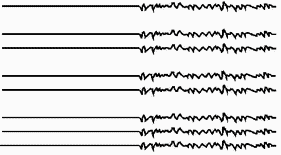
\includegraphics[width=.3\textwidth]{Fig24.png}}
\end{center}

Ce stimuli est disponible pour écoute : \url{http://webpages.mcgill.ca/staff/Group2/abregm1/web/snd/Track24.mp3}} % pour écoute sur le site de Al Bregman dédié à l'ASA. Les détails techniques du processus de synthèse sont renseignés ici : \url{http://webpages.mcgill.ca/staff/Group2/abregm1/web/downloadstoc.htm\#24}.

L'importance perceptive de ce type de modulations dans notre jugement du réalisme d'un stimuli sonore est particulièrement bien exemplifiée par un stimuli synthétique produit par John Chowning. Dans ce stimuli, des sinusoïdes d'amplitude et fréquence au début constantes sont ensuite modulées par un signal synthétique composé d'une composante sinusoïdale (pour le vibrato) auquel se sur-ajoute une composante stochastique. Ce signal modulant est ensuite mis à l'échelle pour chaque harmonique. Il est important de considérer que même si ce signal modulant a été judicieusement choisi, il n'est pas issu d'un processus d'estimation effectué à partir de signaux réels. L'écoute montre clairement que le caractère naturel, voisé, est sensiblement plus élevé avec l'ajout de ces modulations.

\subsection{Modèles perceptifs}

Complétons nos connaissances en prenant un point de vue physiologique. L'étude des éléments physiologiques en charge du traitement de ces modulations est relativement récente car assez complexe à investiguer. On a néanmoins une bonne confiance dans le fait que le système auditif des mammifères dispose d'éléments de traitement dédiés à cette tâche. On peut notamment citer le modèle de Torsten Dau,~\cite{dau1997modeling} qui en plus de la traditionnelle analyse en fréquence effectuée au niveau de la cochlée ajoute une analyse de la modulation d'amplitude. On a donc un modèle temps / fréquence / taux de modulation. Celui de Shihab Shamma~\cite{fritz2003rapid} étend le modèle de Torsten Dau en ajoutant une quatrième dimension : l'échelle, correspondant aux degré de sélectivité des filtres de modulation.

Pour parvenir à ce modèle, Shihab Shamma a étudié certains neurones du cortex auditif primaire du furet, plus particulièrement ce que l'on appelle leur champs de réponse spectro / temporellle ou "spectro-temporal receptive fields" (strf). L'animal est contraint au niveau de la tête, et par opération chirurgicale, une aiguille permettant de mesurer l'activité électrique est insérée dans le crâne de l'animal et judicieusement placée. Par exposition d'un ensemble de stimuli comportant des modulations, il est alors possible de mesurer les strf de certains neurones du cortex auditif. Au vu de ce type de réponses, un modèle de traitement de signal est ensuite proposé.

Dans ce modèle, le signal est donc tout d'abord décomposé sur l'axe fréquentiel. La sortie est un équivalent du spectrogramme qui est ensuite décomposé une nouvelle fois fréquentiellement en temps et en fréquence grâce à des ondelettes bi-dimensionnelles paramétrées avec un facteur d'échelle. La dimension de l'échelle permet de définir le nombre de bandes qui sont conjointement utilisées pour effectuer cette seconde décomposition.

Ces modèles sont bien entendu sujet à débat dans la communauté de neurophysiologie. Par exemple, le facteur d'échelle n'est pas nécessaire dans le modèle de Torsten Dau pour expliquer les données recueillies grâce à son protocole expérimental.

\subsection{\nmu Scattering d'ondelettes}  \label{sec:scattering}

En prenant un point de vue mathématique cette fois-ci, Stéphane Mallat a proposé un modèle conceptuellement proche du modèle computationel des strf proposé par Shihab Shamma. En mathématiques appliquées, et plus particulièrement dans le domaine des sciences des données, on cherche à construire des représentations qui aient de bonnes propriétés d'invariance et de stabilité aux déformations. C'est-à-dire que l'on souhaite que pour une représentation $\Phi(x)$ d'un signal $x$ et d'un signal déformé $\tilde x$ :
\begin{itemize}
  \item $\Phi(\tilde x) = \Phi(x)$ (invariance)
  \item $ \vert \Phi(\tilde x) - \Phi(x) | < \epsilon $ (stabilité)
\end{itemize}
où $\epsilon$ désigne une petite valeur.

Précisons ces notions en prenant quelques exemples. Lorsque l'on cherche à reconnaître l'instrument de musique qui a été utilisé pour jouer une note, on souhaite généralement disposer d'une représentation du signal de cette performance qui soit invariante à certains aspects de la performance comme :
\begin{enumerate}
  \item un changement d'amplitude;
  \item un décalage en temps;
  \item un étirement en temps.
\end{enumerate}
En effet, pour la tâche pré-citée, que la note ait été jouée plus ou moins proche du microphone,~\sidenote{J'écarte ici pour la simplicité du discours les aspects de nuances qui ont une influence non négligeable sur le timbre.} à un instant donné ou quelques secondes plus tard, à une hauteur donnée ou une autre, pour une durée plus ou moins longue ne devrait pas modifier de manière trop conséquente notre représentation.

Sous hypothèse de stationnarité, l'invariance au changement de volume est localement obtenue en normalisant les signaux que l'on souhaite comparer. L'invariance locale à la translation en temps se traduit dans le domaine de Fourier en une invariance à la translation de phase par la prise du module. On souhaite généralement que l'invariance au volume et à la translation soit totale. En ce qui concerne l'invariance à l'étirement temporel, on souhaite généralement plutôt que la représentation soit stable à la déformation.

Il est clairement explicité par Joakim And\'en~\cite{anden2014deep} pourquoi le spectre de magnitude de Fourier d'un signal harmonique n'est pas stable à même un petit étirement temporel. En effet, l'impact de l'étirement selon l'axe des fréquences n'est pas le même. Si un petit étirement déplacera d'une petite quantité les fréquences basses, les fréquences plus élevées le seront beaucoup plus. Prenons l'exemple d'un signal harmonique de fréquence de fondamentale $440$ Hz, un étirement temporel va réduire la valeur de cette fréquence à disons $430$ Hz pour un delta de $10$ Hz. Ce delta sera $n$ fois plus grand pour la $n^{\text{ième}}$ harmonique soit $100$ Hz pour la dixième harmonique. Pour une transformée de Fourier avec une quantification de l'axe fréquentiel d'une dizaine de Hertz, la différence entre les deux spectres va croître très rapidement en fonction du delta car l'énergie des harmoniques supérieures va très rapidement se placer sur des pas de quantification différents de ceux où l'énergie des harmoniques se plaçait initialement.

Pour être plus stable à ce type de déformation, il convient alors de \og délocaliser \fg les hautes fréquences de manière plus conséquente que les basses. Suivant les communautés, on obtient cette délocalisation progressive sur l'axe des fréquences avec des transformées à Q constant, de type tiers d'octave (acoustique), des mels ou des Barks (parole)\marginnote[0cm]{Ce résultat est, à mon sens, d'importance, car il permet de placer un cadre mathématique pour mieux expliquer l'utilité d'un axe fréquentiel logarithmique qui a été empiriquement vérifié dans de nombreux domaines du traitement de l'audio et motivé jusqu'ici par des arguments essentiellement neuro mimétiques.}.

En se plaçant dans le cadre du scattering d'ondelettes, dont le schéma fonctionnel est montré sur la Figure \ref{fig:scat}, on obtient ce type de représentation en délocalisant en temps toutes les bandes de fréquence du module de la transformée en ondelettes $\psi_1$ par l'application d'un filtre moyennant $\phi$ pour obtenir les coefficients de scattering au premier ordre $S_1$ :

\begin{equation}
S_1{x}(t, \lambda_1)
= \vert {x} \ast {\psi_{\lambda_1}} \vert \ast \phi(t)\mbox{.}
\end{equation}

Ceci induit une perte d'information qu'il convient de compenser. Le principe du scattering d'ondelettes permet de répondre élégamment à ce problème en cascadant des opérations de décomposition et en utilisant chaque niveau de décomposition pour produire une représentation compacte et informative. Ainsi, on obtient au second ordre :

\begin{equation}
S_2{x}(t, \lambda_1, \lambda_2)
= \vert \vert {x} \ast {\psi_{\lambda_1}} \vert \ast {\psi_{\lambda_2}} \vert \ast \phi(t)\mbox{.}
\end{equation}

Comme le montre la Figure \ref{fig:scat}, le scattering dissocie décomposition et représentation, ce qui permet de préserver certaines propriétés d'intérêt comme, par exemple, l'inversibilité pour la décomposition sous certaines conditions et la stabilité pour la représentation.

\begin{figure}[t]
  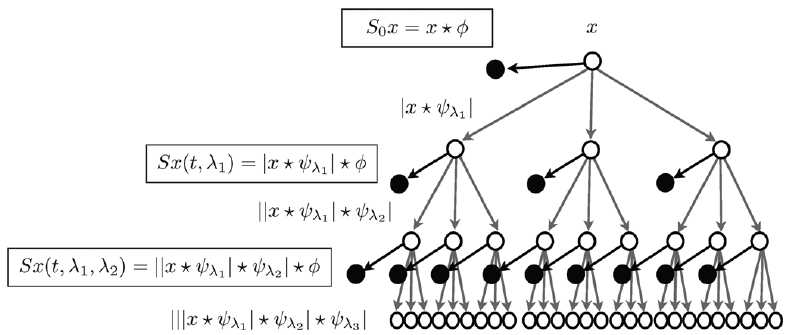
\includegraphics[width=\textwidth]{scattering.png}
  \caption{Propagation du signal au travers du scattering d'ondelettes au premier et second ordre (figure issue de la référence \no 59).}
  \label{fig:scat}
\end{figure}

La sortie du filtre moyenneur au premier ordre est donc équivalent à une transformée à Q constant. En décomposant les sorties rectifiées du premier banc de filtres en ondelettes $\psi_{\lambda_1}$ avec un autre banc de filtres en ondeletes $\psi_{\lambda_2}$, on capte alors l'information de modulation d'amplitude, \textit{i.e.} comment l'énergie fluctue dans une même bande fréquence. On a vu précédemment l'importance de ce type de modulation pour la perception. Il est donc opportun de d'étudier l'apport du second ordre pour une représentation riche du signal sonore.  %\marginnote{Le processus de cascade. Le troisième ordre est conceptuellement difficile à appréhender et a encore été peu étudié, pour les raisons suivantes 1) pratique : l'énergie au troisième ordre est très faible, 2) neuro-mimétique : aucun modèle perceptif n'explicite un troisième ordre de traitement.}.


\begin{figure*}[t]
  \begin{tabular}{cc}
    (1)  &   (2)\\ \\
      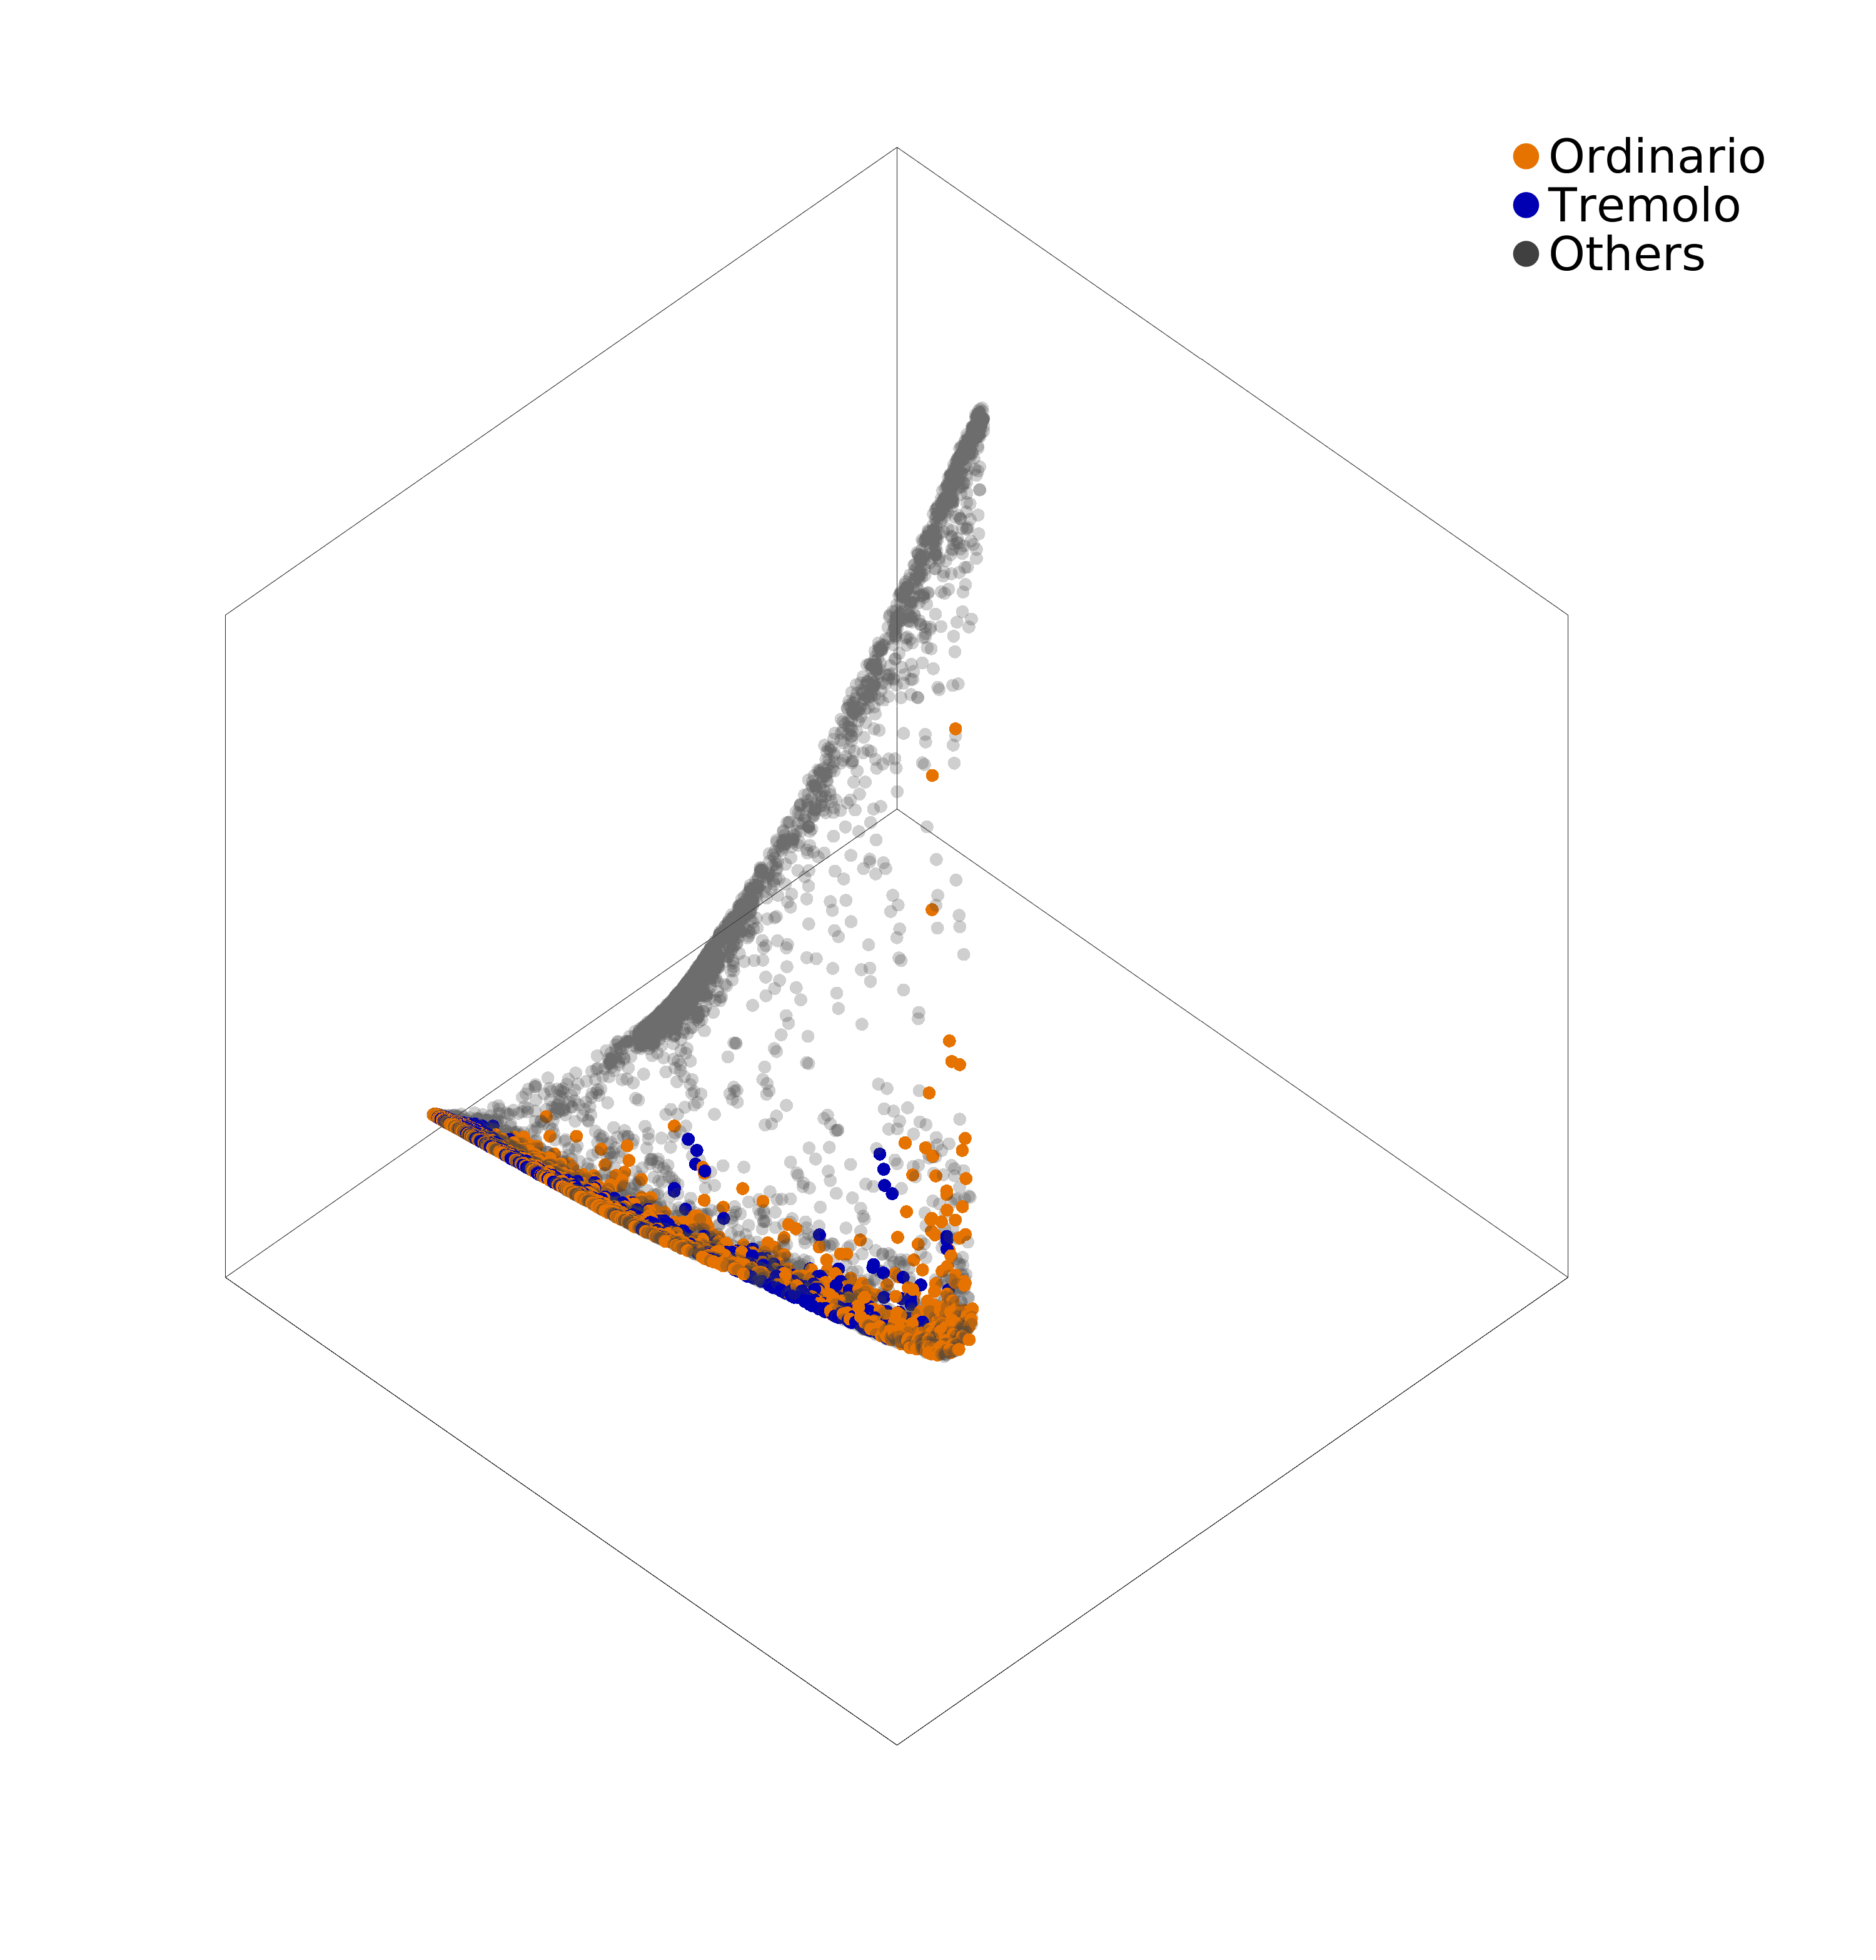
\includegraphics[width=.5\textwidth]{mf_tech_two_dmap.png} &
      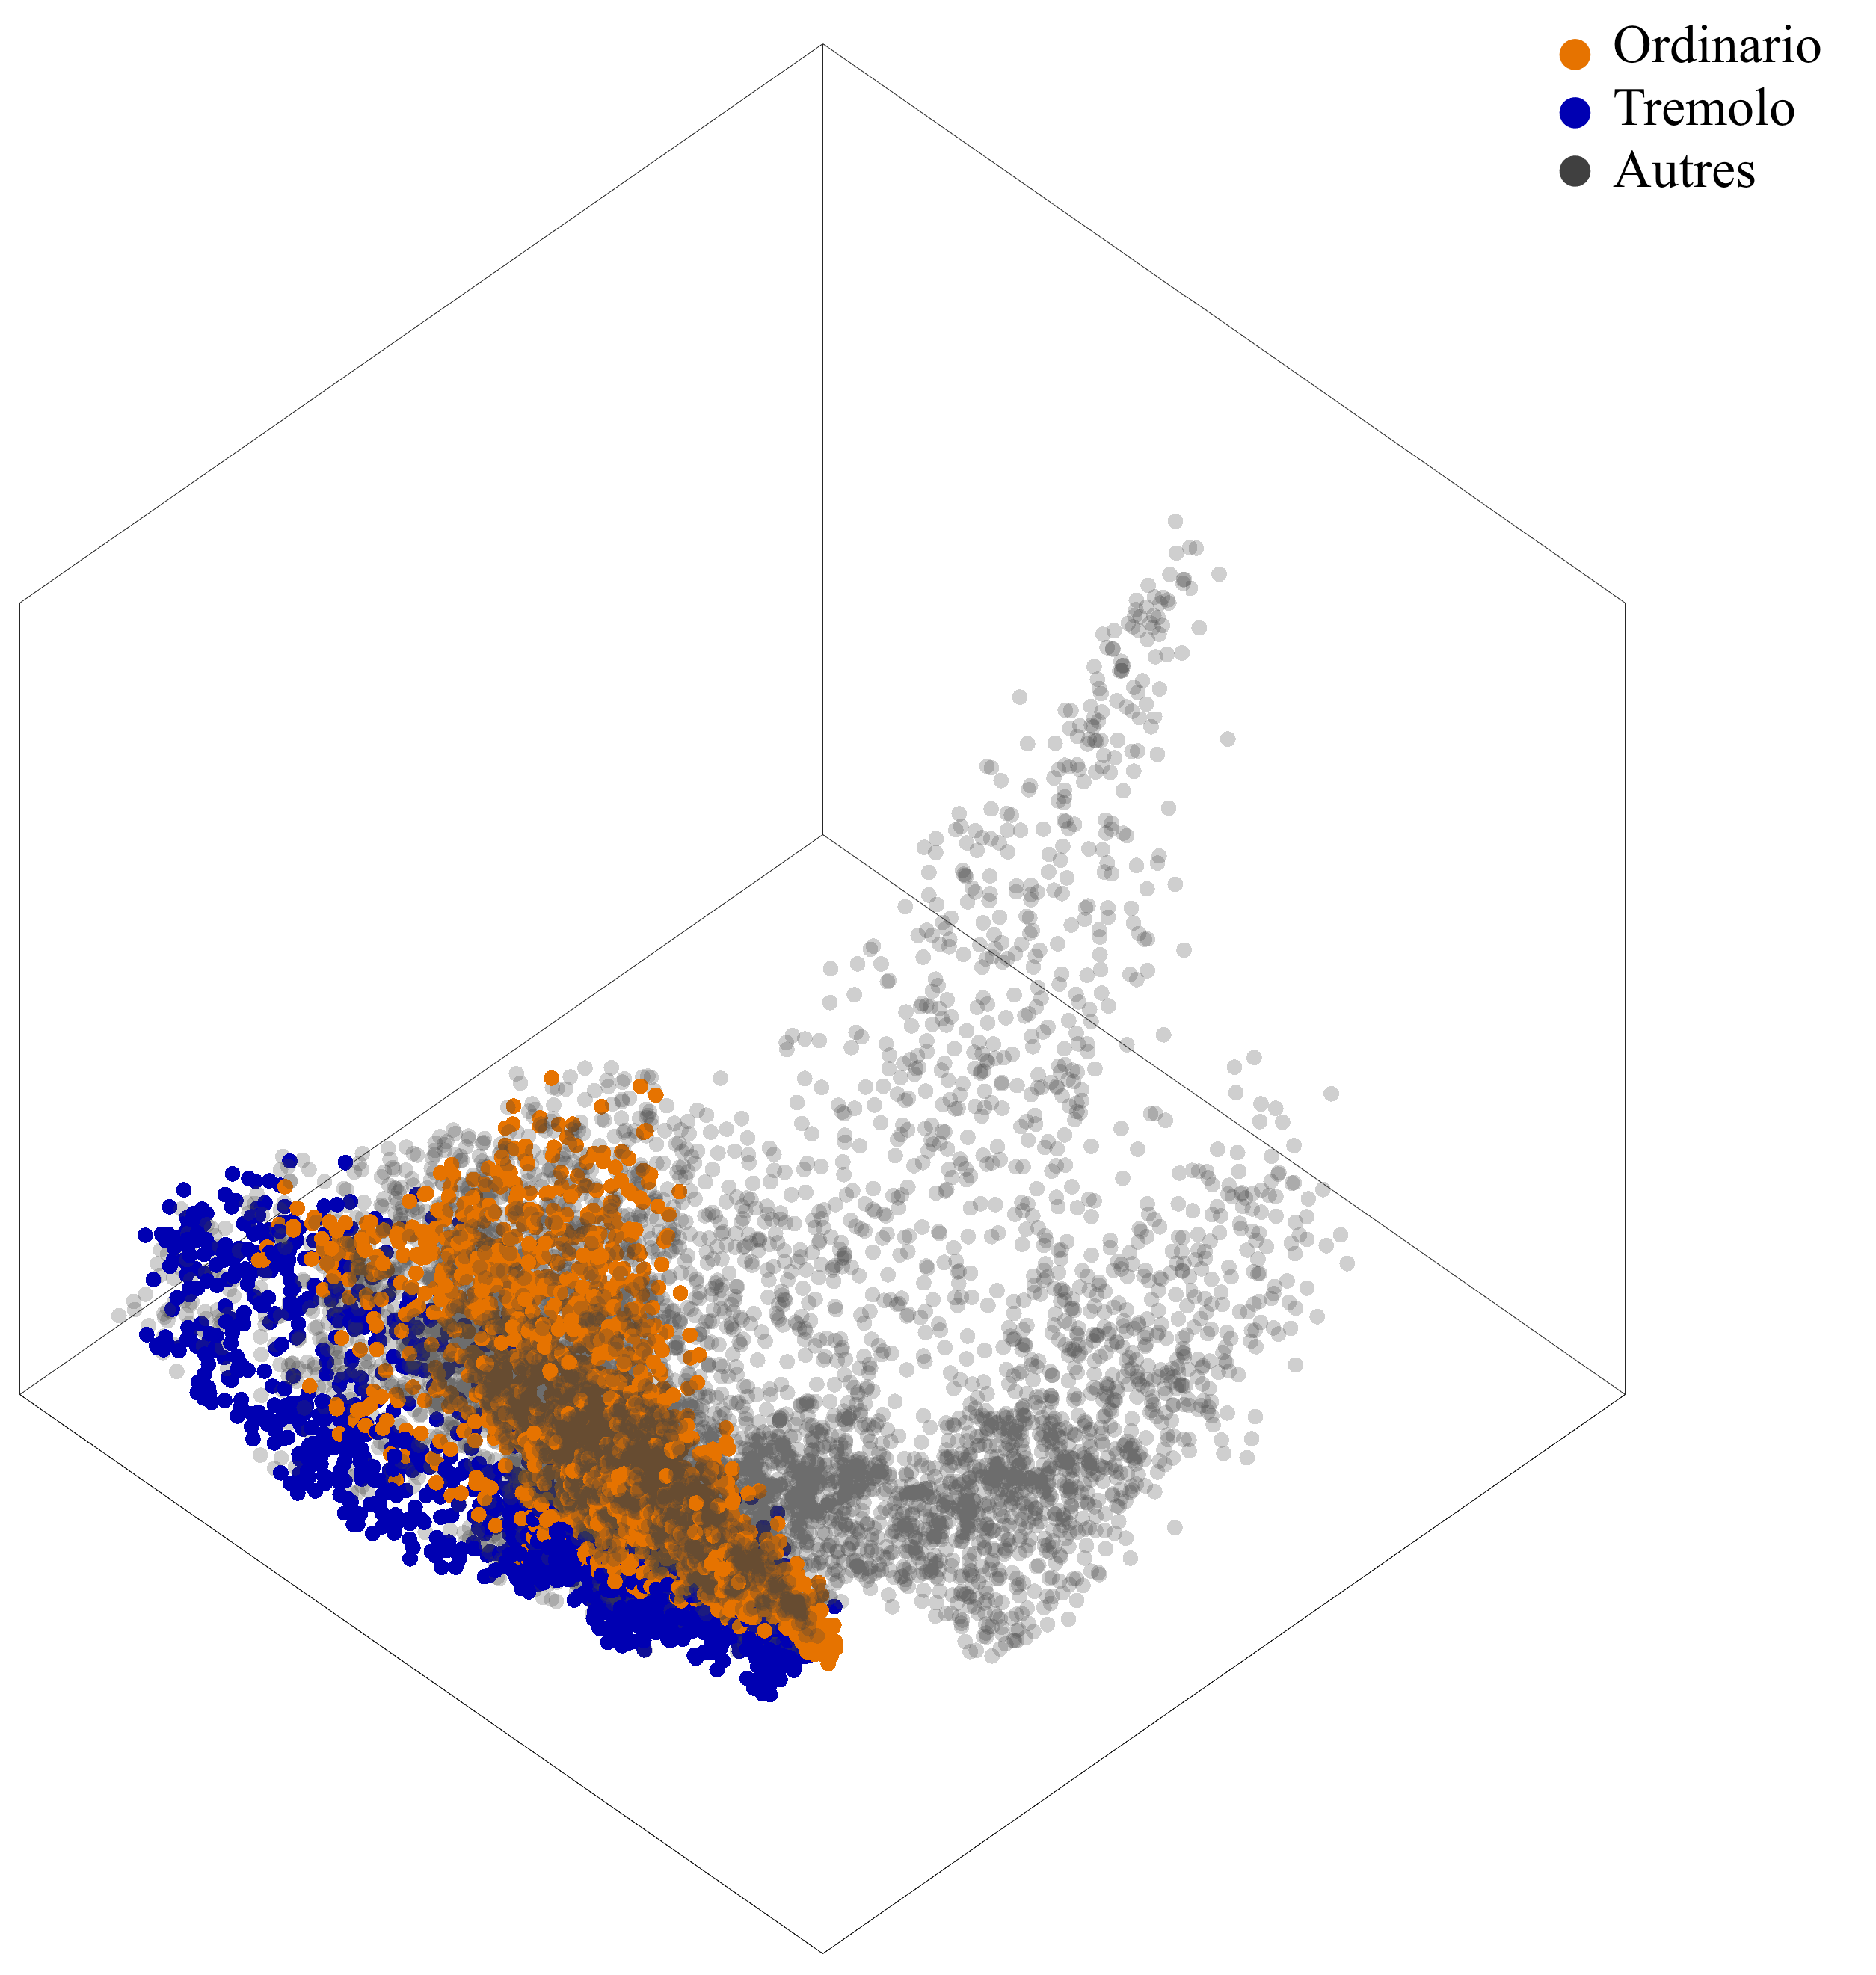
\includegraphics[width=.5\textwidth]{sc_tech_two_dmap.png}
  \end{tabular}
  \begin{center}
  \end{center}
  \label{fig:dm}
  \caption{"Diffusion maps" obtenues à partir du scattering d'ondelettes à l'ordre 1 et 2.}
\end{figure*}


Son apport a été démontré expérimentalement pour de nombreuses tâches de modélisation. Nous avons complété cet effort de recherche en considérant des sons d'instruments de musique du répertoire avec des modes de jeux étendus.~\cite{lostanlen2018extended} En effet, si la reconnaissance de l'instrument est considérée comme un problème résolu par une représentation à Q constant, la reconnaissance du mode de jeu nécessite d'être à même de modéliser des éléments de modulations qui ne sont pas aisément capturés par une représentation à Q constant ou un scattering d'ondelettes à l'ordre un. En considérant la méthode des "diffusion maps"~\cite{coifman2005geometric} pour obtenir un espace de projection à 3 dimensions à partir respectivement d'une représentation à Q constant et du scattering d'ondelettes à l'ordre 2, on note par exemple que le mode de jeu \textsl{tremolo} est mieux distingué du mode de jeu ordinaire dans la seconde projection, voir Figure \ref{fig:dm}.

On est donc en mesure de correctement modéliser les modulations d'amplitude. Pour permettre de modéliser des modulations sur l'axe fréquentiel, il est nécessaire de considérer des ondelettes bi-directionnelles sur le plan temps / fréquence, ce qui rend le modèle conceptuellement plus proche du modèle perceptif de Shihab Shamma.~\cite{8721532}

En terme d'architecture, le scattering d'ondelettes suit une organisation de type réceptive, 1) fréquence et 2) temps ou fréquence / temps ensuite. On verra dans la partie suivante un modèle prenant une approche de type source / filtre donc temps puis fréquence  et qui est à ce titre plus proche d'un modèle de production.

\section{ \nmu Synthèse modale}


\marginnote[0cm]{
  \scalebox{.7}{
  
\begin{tikzpicture}[
nonterminal/.append style={join=by ->},
tip/.style={->,shorten >=1pt},every join/.style={rounded corners},
terminal/.style={
% The shape:
rectangle,minimum size=6mm,rounded corners=1mm,
% The rest
very thick,draw=black!50,
top color=white,bottom color=black!10,
font=\ttfamily},
point/.style={circle,fill=black,minimum size=2pt},
%every node/.style=draw,
line/.style ={draw, thick, -latex',shorten
  >=2pt}]
%%%%%%%%%%%%%%%%%%%%%%%%%%%%%%%%%%%%%%%%%%%%%%%%%%%%%%%%%%%

\matrix [column sep=5mm,row sep=5mm]
{
\node [point] (p1) {} ; & \node (p2) {} ; & \node [terminal] (ma) {Analyse modale} ; &&& \node (e4) {} ; \\
&& \node [terminal] (md) {Déconvolution modale} ; & \node [terminal]  (is) {Sélection des impacts}
; && \node (e3) {} ; \\
&&& \node [terminal] (im) {Modélisation} ; && \node (e2) {} ; \\
&&& \node [terminal] (id) {Deconvolution} ; & & \node (e1) {} ;  \\
};

\begin{scope}[every path/.style=line]
\path (p1) -- node [above] {$s[n]$} (ma);
\path (p2) |- (md);
\path [dashed] (ma)  -- (md);
\path [dashed] (ma) --  node [above] {$a_k, f_k$} (e4);
\path (md) |- (id);
\path (md) -- node [above] {$e[n]$} (is);
\path (is) -- (im);
\path (is) --  node [above] {$i[n]$} (e3);
%\path (im) --  node [above] {$m(n)$} (e2);
\path (im) -- node [right] {$m[n]$} (id);
\path (id) -- (e1);
\path (id) -- node [above] {$d[n]$} (e1);
\end{scope}

\end{tikzpicture}
}
Schéma de traitement de la phase d'analyse d'un modèle de synthèse modale pour les sons de roulement. Les traits pleins désignent des signaux, les traits pointillés désignent des paramètres.
}


En se référant plutôt aux processus physiques de production sonore, les approches modales permettent de proposer des modèles qui sont à la fois efficaces et effectifs. Ces modèles se basent sur un modèle de production de type source / filtre, où la source est généralement décrite en terme de propriétés temporelles, et le filtre en terme de propriétés fréquentielles. Pour un signal de parole, on considèrera que la source peut être soit un train d'impulsions résultant de l'ouverture périodique des plis vocaux pour la production des sons voisés (voyelles) soit un signal stochastique résultant de la compression du flux respiratoire pour la production des plosives ou sifflantes (consonnes).

Le modèle source / filtre décorrèle donc naturellement la contribution de l'excitateur et celle du résonateur, ce qui est particulièrement attrayant lorsque l'on recherche un modèle de son permettant une bonne capacité d'interaction. Pour peu que les modèles utilisés pour les deux parties (source et filtre) soient bien adaptés, on obtient des modèles de sons qui sont souvent fidèles et particulièrement expressifs.~\cite{aramaki2006analysis}

Nous avons étudié ce type de modèle pour la synthèse de sons de roulements d'une bille sur une plaque. Ces sons présentent un challenge pour ce type de synthèse car l'interaction entre la bille et la surface sur laquelle elle roule est complexe. Néanmoins, ce type de modèle adapté au problème~\cite{LagrangeTasslp10} a donné des résultats encourageants.~\cite{Murphy11a}

Dans cette contribution, l'étape d'analyse consiste à identifier les composantes résonantes paramétrées par leur fréquence de résonance $f_k$ et leur amplitude $a_k$ et les utiliser pour opérer une déconvolution du signal enregistré $s[n]$. Le résiduel $r[n]$ de cette déconvolution  permet d'identifier une forme typique $i[n]$ de l'impact de la bille avec la plaque la position des impacts. Cette forme est alors utilisée pour déconvoluer $r[n]$ et ainsi obtenir un signal $d[n]$ essentiellement composé de pics indiquant la position et la puissance des impacts de la bille sur la plaque.

La source est modélisée comme une série d'impacts dont l'amplitude est modélisée par une distribution exponentielle paramétrée par $\lambda_a$  et l'intervalle de temps entre deux impacts par une distribution gamma paramétrée par $k_i$ et $\theta_i$. Ces paramètres sont estimés à partir de $i[n]$.

En remarquant fort justement que, lorsque la bille impacte fortement la plaque sur laquelle elle roule, l'intervalle entre cet impact et le suivant augmente, Simon Conan a proposé un modèle amélioré où ces variables sont modélisées de manière conjointe.~\cite{conan2014synthesis}

Ce type d'approche se situant à l'intersection entre modélisation statistique et modélisation physique possède deux propriétés d'intérêt, avec en premier lieu, la causalité. Au niveau du modèle de synthèse, un échantillon est strictement considéré comme une composante des échantillons précédents. En second, cette approche met l'accent sur les propriétés de filtrage des composantes modales, il ne s'agit pas ici de synthétiser un signal riche à partir d'une représentation complète du signal, mais plutôt d'exploiter un modèle source / filtre avec une implantation dédiée de ces deux modules en fonction de la tâche visée.

\marginnote[-2cm]{
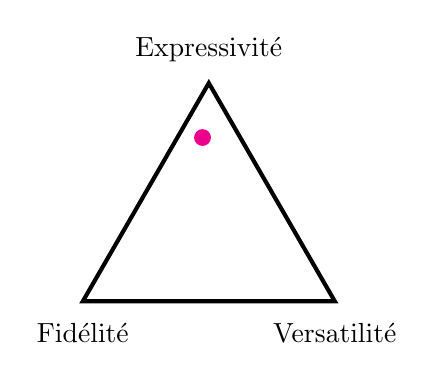
\begin{tikzpicture}[scale=0.8, label distance=1.5mm]
  \coordinate[label=below:Fidélité]  (A) at (0,0);
  \coordinate[label=below:Versatilité] (B) at (4,0);
  \coordinate[label=above:Expressivité] (C) at (2,3.464);
  \draw [line width=1.5pt] (A) -- (B) -- (C) -- cycle;
  \draw [magenta, fill=magenta, line width=1.5pt] (1.9,2.6) circle [radius=.1 cm]; % modal
  \end{tikzpicture}
  Le modèle modal est particulièrement expressif et fidèle pour un champ assez réduit de signaux sonores.
}

Malgré toutes ces bonnes propriétés, de manière peut-être encore plus marqué que pour les modèles sinusoïdaux à long terme, la versatilité reste malheureusement en deçà, car le changement de structures pour la source et le filtre ainsi que leurs modes d'interactions nécessitera le plus souvent des adaptations d'ordre computationel si ces changements sont conséquents. En particulier, les interactions non linéaires sont difficiles à modéliser en raison de manque d'outils d'estimation génériques.

%Même si ce type d'approche est utilisée de manière assez marginale, elle garde à mon sens un intérêt pour mettre en perspective les approches modernes discutées dans la suite.

\section{ \nmu Discussion}

\marginnote{
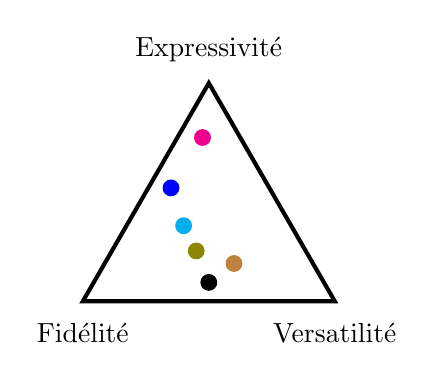
\begin{tikzpicture}[scale=0.8, label distance=1.5mm]
  \coordinate[label=below:Fidélité]  (A) at (0,0);
  \coordinate[label=below:Versatilité] (B) at (4,0);
  \coordinate[label=above:Expressivité] (C) at (2,3.464);
  \draw [line width=1.5pt] (A) -- (B) -- (C) -- cycle;
  \draw [black, fill=black, line width=1.5pt] (2,.3) circle [radius=.1 cm]; % raw
  \draw [olive, fill=olive, line width=1.5pt] (1.8,.8) circle [radius=.1 cm]; % spec
  \draw [brown, fill=brown, line width=1.5pt] (2.4,.6) circle [radius=.1 cm]; % wavelets
  \draw [cyan, fill=cyan, line width=1.5pt] (1.6,1.2) circle [radius=.1 cm]; % sct
  \draw [blue, fill=blue, line width=1.5pt] (1.4,1.8) circle [radius=.1 cm]; % slt
  \draw [magenta, fill=magenta, line width=1.5pt] (1.9,2.6) circle [radius=.1 cm]; % modal
  \end{tikzpicture}

  \vspace{.3cm}

  \begin{tabular}{cl}
    \tikz\draw[black,fill=black] (0,0) circle (.1 cm); & Forme d'onde \\
    \tikz\draw[olive,fill=olive] (0,0) circle (.1 cm); & Spectrogramme \\
    \tikz\draw[brown,fill=brown] (0,0) circle (.1 cm); & Ondelettes \\
    \tikz\draw[cyan,fill=cyan] (0,0) circle (.1 cm); & Sinusoïdes à court terme \\
    \tikz\draw[blue,fill=blue] (0,0) circle (.1 cm); & Sinusoïdes à long terme \\
    \tikz\draw[magenta,fill=magenta] (0,0) circle (.1 cm); & Approches modales
  \end{tabular}
}

Si l'on prend une vue d'ensemble des différents compromis pris par les modèles de sons précédemment décrit, on voit qu'il existe des compromis équilibrés entre fidélité et expressivité au détriment de la versatilité et des compromis équilibrés entre fidélité et versatilité au détriment de l'expressivité, avec un \og juste milieu \fg occupé par le spectrogramme. Le grand défi de la modélisation sonore est donc de proposer des approches qui puissent se placer dans un compromis entre versatilité et expressivité avec une fidélité qui reste raisonnable.

\begin{table}
  \begin{tabular}{cccc}
    & fidélité & versatililité & expressivité  \\
  multirésolution & \blackdot  & \blackdot & \\
  causalité & \blackdot  &  & \blackdot \\
  non linéarité & \blackdot  & \blackdot & \\
  dimensionalité réduite &  & &  \blackdot \\
  contrôle lent &  & &  \blackdot
  \end{tabular}
  \vspace{.5cm}
  %\caption{Relations entre fonctionalités et objectifs.}
\end{table}



Au vu des arguments discutés durant cette présentation, quelques éléments se révèlent incontournables pour espérer relever ce défi. Tout d'abord, le modèle doit inclure des aspects de \textbf{multirésolution} pour être à même de contourner au mieux les contraintes posées par le principe d'incertitude. Il me paraît également incontournable que le modèle soit \textbf{causal}. La non causalité permet certes une plus grande flexibilité algorithmique et facilite souvent l'identification. Pour des applications de génération en revanche, la perte de la causalité amène malheureusement des approximations qui sont souvent détrimentaires à la fidélité, car le processus physique qui a produit le signal sonore est lui causal.

Ensuite, de nombreuses étapes de la propagation des ondes sonores peuvent être considérés comme des systèmes linéaires. Néanmoins, il s'avère critique pour la qualité perceptive des signaux produits que le modèle puisse également modéliser des processus \textbf{non linéaires} pour accéder à une grande versatilité. Cela pose bien entendu le problème du contrôle, les structures algorithmiques non linéaires étant plus complexes à manipuler. Pour des raisons d'expressivité, il est ensuite nécessaire que le contrôle soit aisé, ce qui amène d'autres contraintes en terme d'espace de description. Il est souhaitable qu'il soit d'une \textbf{faible dimensionalité} et que son \textbf{échantillonnage temporel} soit sensiblement plus \textbf{lent} que celui du signal.

La plupart des outils présentés dans ce chapitre relèvent du domaine du traitement du signal. Il est néanmoins remarquable que, pour la plupart des contributions récentes en sciences des données, les éléments déterminants au progrès des systèmes relèvent principalement de l'apprentissage automatique. Même si ces disciplines partagent de nombreux fondements mathématiques en terme de modélisation de l'information, il est important de bien comprendre les différences de méthodologie. Ce sujet passionnant nécessiterait une étude complète, je me contenterai donc ici d'une caricature pour les besoins du propos. Dans une approche traitement du signal, l'expert met en place une structure algorithmique avec un nombre de degrés de liberté réduit qui lui permet d'envisager un paramétrage manuel ou par le biais d'un plan expérimental relativement réduit. Dans l'approche apprentissage, le nombre de degrés de liberté devient tellement grand que les mécanismes d'optimisation automatique deviennent indispensables. Il est bien entendu que ces méthodes d'optimisation ont leurs paramètres, qui doivent être également choisies avec soin.

La place de l'apprentissage dans les chaînes de prise de décision n'a fait que grandir ces dernières années. Ce mouvement sonne-t-il le glas du traitement du signal ? En terme de composant algorithmique indépendant c'est en effet probable. En terme de discipline, de nombreuses opportunités sont ouvertes. En effet, les avancées obtenues grâce aux mécanismes d'apprentissage relèvent pour beaucoup de démarches inductives. A ce jour, la compréhension et la formalisation de la manière dont l'information est traitée dans ces structures algorithmiques complexes est donc largement incomplète.

Finalement, qu'il s'agisse de modèles de perception, de modèles d'apprentissage, ou de modèles de production, \og tout est filtrage \fg. Il est pour cette raison prédictible que les contributions à l'interface de ces deux disciplines constitueront des avancées significatives aux défis relevant du domaine des sciences des données.~\cite{mallat2016understanding}

Dans cette quête, l'étude des signaux temporels comme les signaux sonores permet de se confronter aux besoins pré-cités: multirésolution, causalité, non-linéarité. Ces verrous sont au c\oe{}ur des problématiques identifiées par la communauté des sciences des données. Par exemple, les avancées récentes par réseaux de neurones convolutionels récurrents pour la synthèse de signaux sonores basés échantillons~\cite{wavenet} proposent des architectures qui possèdent de manière remarquable les conditions nécessaires pré-citées et devraient obtenir en théorie un excellent compromis entre fidélité et versatilité. La possibilité de conditionner le réseau de manière assez flexible donne en outre de bons espoirs en terme d'expressivité.

Est-ce que l'intérêt de ce type d'architecture se confirmera en amenant des réponses aux défis identifiés dans ce chapitre ? Répondre à cette question ouvre un champ d'expérimentation passionnant pour l'expérimentateur qui se doit d'être guidé par une approche méthodologique rigoureuse, et fondée sur des questionnements scientifiques clairement explicités.
